\documentclass[8pt]{beamer}
\usetheme{default} % Very simple theme
\usecolortheme{dove} % Minimalist grayscale colors
\setbeamertemplate{navigation symbols}{} % Remove navigation bar

% Define brand-like colors
\definecolor{myblue}{RGB}{0, 102, 204}    % Blue for standard blocks
\definecolor{mygreen}{RGB}{0, 153, 0}     % Green for example blocks
\definecolor{myred}{RGB}{204, 0, 0}       % Red for alert blocks
\definecolor{myorange}{RGB}{255, 128, 0} % For \emph

% Accent color for titles, bullets, etc.
\setbeamercolor{structure}{fg=myblue}

% Block colors
\setbeamercolor{block title}{bg=myblue, fg=white}
\setbeamercolor{block body}{bg=blue!5, fg=black}

\setbeamercolor{exampleblock title}{bg=mygreen, fg=white}
\setbeamercolor{exampleblock body}{bg=green!5, fg=black}

\setbeamercolor{alertblock title}{bg=myred, fg=white}
\setbeamercolor{alertblock body}{bg=red!5, fg=black}
\setbeamercolor{alerted text}{fg=myred}

% Optional: color for \example text
\setbeamercolor{example text}{fg=mygreen}

% Custom emph (orange text instead of italic)
\let\oldemph\emph
\renewcommand{\emph}[1]{\textcolor{myorange}{#1}}


\usepackage{graphicx} % Package for images
\usepackage{amsmath} % Package for images
\graphicspath{{figs/}} % Path to your figures directory
\usepackage{array}  % For better column spacing
\usepackage{caption} % Required for \captionof

% Title Information
\title{Stochastic methods in water resources}
\subtitle{Lecture 4: Moments, characteritics function, known probability distributions, bivariate probability distributions}
\author{Luis Alejandro Morales, Ph.D.}
\institute{Universidad Nacional de Colombia} %// Department of Civil and Agriculture Engineering}
\date{\today}

\begin{document}

% Title Slide
\begin{frame}
    \titlepage
\end{frame}

%-------
% From Diaz-granados
\section{Measures of probability distribution}
\subsection{Expected value}
\begin{frame}{Expected value}
    The measures or descriptors of a random variable determine important features of their behaviour and thus describe the \emph{pmfs} and \emph{pdfs}. The descriptors are defined upon the \emph{pmfs} o \emph{pdfs} and are known as the statistics of the random variable. 
    \begin{block}{Expected value}
        If $X$ is a discrete random variable and $g(x)$ is a function of the random variable, the \alert{expected value} of $g(x)$ is:
        \[
            E\left[g(x)\right] = \sum g(x_i) p_X(x_i)
        \]
        If $X$ is continuos, \alert{expected value} is:
        \[
            E\left[g(x)\right] = \int_{-\infty}^{\infty} g(x) f_X(x)
        \]
        These equations indicate that the expected value or average of a random variable $X$ is computed by weighting the random variable function $g(X)$ with the \emph{pmf} or the \emph{pdf}. Some of the properties of the expected value operator, $E$, are:
        \begin{align*}
            E(a) &= a, \text{ when $a$ is constant} \\
            E\left[a g(x) \right] &= a E\left[g(x) \right], \text{ when $a$ is constant} \\
            E\left[a g_1 (x) + b g_2 (x) \right] &= a E\left[g_1 (x) \right] + b E\left[g_2 (x) \right], \text{ if $a$ y $b$ are constants} \\
            E\left[g_1 (x) \right] &\leq E\left[g_2 (x) \right],  \text{ if $g_1(x) \geq g_2(x)$}
        \end{align*}
    \end{block}
\end{frame}

\subsection{Moments}
\begin{frame}{Moments}
    
    \begin{block}{Moments}
        The \alert{moments} are a family of averages or expected values of a random variable used to describe its behaviour. It is common to characterize a \emph{pmf} or a \emph{pdf} using its main moments. If $\mu_r^*$ represents the moment of order $r$ around the point $a$, this is defined  for a discrete variable as:
        \[
            \mu_r^* = E \left[(X - a)^r \right] = \sum_{\text{todo $x_i$}} (x_i - a)^r p_X (x_i) 
        \]
for a continuous variable:
        \[
            \mu_r^* = E \left[(X - a)^r \right] = \int_{-\infty}^{\infty} (x- a)^r f_X (x) dx
        \]
        where $r$ is an positive number.  The most known moments to describe $pmfs$ or $pdfs$ are the \alert{mean} ($\mu_X$), the \alert{variance} ($s_X = \sigma_X^2$) and the asymmetry  $\gamma$.
    \end{block}
    \vspace{-6pt}
    \begin{block}{Mean, $\mu_X$}
        The \alert{mean} is the first moment ($r = 1$) with respect to the origin ($a = 0$). It is measure that describe the central tendecy of the random variable. The \alert{mean} has the same units that $X$. This is defined as:
\begin{minipage}[t]{0.48\textwidth}
\centering
\textbf{Discrete random variable $X$}
\[
\mu_X = E \left[ X \right] = \sum_{\text{todo $x_i$}} x_i p_X (x_i)
\]
\end{minipage}
\hfill
\begin{minipage}[t]{0.48\textwidth}
\centering
\textbf{Continuous random variable $X$}
\[
\mu_X = E \left[ X \right] = \int_{-\infty}^{\infty} x f_X (x) dx
\]
\end{minipage}
\end{block}
\end{frame}

\begin{frame}{Moments}
    \begin{block}{Variance, $\sigma_X^2$}
        The \alert{variance} is the second moment ($r = 2$) with respect to the $a = \mu_X$. The \alert{variance} describes the variability of a random variable $X$ around their expected value $\mu_X$.
\begin{minipage}[t]{0.49\textwidth}
\centering
\textbf{Discrete random variable $X$}
\begin{align*}
    \sigma_X^2 &= E \left[ (X - \mu_X)^2 \right] \\ 
               &= \sum_{i=1}^n (x_i - \mu_X)^2 p_X (x_i)
\end{align*}
\end{minipage}
\hfill
\begin{minipage}[t]{0.49\textwidth}
\centering
\textbf{Continuous random variable $X$}
\begin{align*}
    \sigma_X^2 &= E \left[ (X - \mu_X)^2 \right] \\
               &= \int_{-\infty}^{\infty} (x - \mu_X)^2 f_X (x) dx
\end{align*}
\end{minipage}
The larger $\sigma_X^2$, the larger the dispersion of $X$ aroung $\mu_X$. According to the properties of $E$ discussed above, one can demostrate that:
\[
    \sigma_X^2 = E \left[ (X - \mu_X)^2 \right] = E [X^2] - \left( E[X] \right)^2
\]
The \alert{standard deviation}, $\sigma_X$, is defined as:
\[
    \sigma_X = \sqrt{\sigma_X^2}
\]
where $\sigma_X$ has the same units of $X$ and thus facilitate the understanding of the dispersion of $X$ around $\mu_X$. The relative measure of dispersion with respect to $\mu_X$ is the \alert{coefficient of variation} defined as:
\[
    V_X = \frac{\sigma_X}{\mu_X}
\]
\end{block}
\end{frame}

\begin{frame}{Moments}
    \begin{block}{Asymmetry, $\gamma$}
The \alert{asymmetry}, $\gamma$,  is the third moment ($r=3$) around the mean ($a = \mu_X$). The definition is:

\begin{minipage}[t]{0.49\textwidth}
\centering
\textbf{Discrete random variable $X$}
\begin{align*}
    \gamma &= E \left[ (X - \mu_X)^3 \right] \\ 
               &= \sum_{i=1}^n (x_i - \mu_X)^3 p_X (x_i)
\end{align*}
\end{minipage}
\hfill
\begin{minipage}[t]{0.49\textwidth}
\centering
\textbf{Continuous random variable $X$}
\begin{align*}
    \gamma &= E \left[ (X - \mu_X)^3 \right] \\
               &= \int_{-\infty}^{\infty} (x - \mu_X)^3 f_X (x) dx
\end{align*}
\end{minipage}
$\gamma$ is a measure of the \emph{pmf} or \emph{pdf} symmetry. Based on these equations, the nondimensional asymmetry coefficient is defined as:
\begin{align*}
\gamma_1 &= \frac{E \left[ (X - \mu_X)^3 \right]}{\sqrt{\left[ E \left[ (X - \mu_X)^2 \right]\right]^3}} \\
         &= \frac{E \left[ X^3 \right] - 3E\left[ X^2 \right] \mu_X + 2 \mu_X^3 }{\left( E\left[ X^2 \right] - \mu_X^2 \right)^\frac{3}{2}}
\end{align*}
As you can see in the equation above, the numerator is the central moment of third order ($r=3$) and the denominator is $\sigma_X$ raised to the power of 3. Note that $\gamma_1$ have the same sign that $\gamma$. For symetrical distribution, $\gamma \approx 0$.  
\end{block}
\end{frame}


\begin{frame}{Moments}
    \begin{block}{Quantiles, $q$}
        The $q$-esimo quantile, $q$, of a random variable $X$, is defined as the smallest  number $\xi$ that satisfy the inequality $F_X (\xi) \geq q$. For a continuos variable, $\xi$ sastisfy $F_X (\xi) = q$ and the quantile is the value of $X$ that is exceeded with a probability of $(1-q)$. Convesely, the quantile can be written as $q = x(F)$ or $q = x[F_X (x)]$. Accordingly, the mediana is the 0.5 quantile, written as $\xi_{0.5}$. A quantile $q$ can be defined as $\xi_q = F_X^{-1} (q)$. The most common $q$ are the quartiles $\xi_{0.25}$, $\xi_{0.5}$ and $\xi_{0.75}$. 
\end{block}
\vspace{-6pt}
    \begin{exampleblock}{Daily evaporation}
        Suppose that the pdf of the evaporation $V$ for any day of the year is defined as:
\[
f_V (v) = 
\left\{
\begin{array}{l}
    0.125 \text{, if } 0.5\leq v \leq 8.5 \ mm/day  \\
    0 = \text{ otherwise} 
\end{array}
\right.
\]

Estimate the main moments. 

\begin{minipage}[t]{0.44\textwidth}
\centering
\textbf{Mean $\mu_V$}
\begin{align*}
    \mu_V&= E \left[ V \right] = \int_{-\infty}^{\infty}v f_V(v) dv \\
         &= \int_{0.5}^{8.5} 0.125 v dv\\ 
               &= 0.0625 v^2 \Big|_{0.5}^{8.5} = 4.5 mm/day
\end{align*}
\end{minipage}
%\hfill
\begin{minipage}[t]{0.44\textwidth}
\centering
\textbf{Variance $\sigma_V^2$}
\begin{align*}
    \sigma_V&= E \left[ (v -\mu_V)^2 \right] \\
            &= \int_{-\infty}^{\infty} (v-\mu_V)^2 f_V(v) dv \\
            &= 0.125 \int_{0.5}^{8.5}  (v-4.5)^2 dv\\ 
            &= \frac{0.125}{3} \left[ (v-4.5)^3 \right] \Big|_{0.5}^{8.5} = 5.33 mm^2 /day^2
\end{align*}
\end{minipage}
    \end{exampleblock}
\end{frame}

\begin{frame}{Moments}
    \begin{exampleblock}{Daily evaporation}
\begin{minipage}[t]{0.39\textwidth}
\centering
\textbf{Standard deviation $\sigma_V$}
\[
    \sigma_V = \sqrt{\sigma_V^2} = \sqrt{5.33} = 2.31 mm/day
\]
\textbf{Quantile $\xi$}

From the $F_V (v) = 0.125v - 0.0625$ and regarding that $\xi_q = F_V^{-1} (q)$, one has that $\xi_q = 8(q + 0.0625)$. So $\xi_{0.1} = 1.3$ and $\xi_{0.5} = 4.5$ (the mediana). The interquartile range is $q_r = \xi_{0.75} - \xi_{0.25} = 6.5 - 2.5 = 4$. 
\end{minipage}
\hfill
\begin{minipage}[t]{0.59\textwidth}
\centering
\textbf{Assymetry $\gamma$}
\begin{align*}
    \gamma &= E \left[ (v -\mu_V)^3 \right] = \int_{-\infty}^{\infty} (v-\mu_V)^3 f_V(v) dv \\
            &= 0.125 \int_{0.5}^{8.5}  (v-4.5)^3 dv\\ 
            &= \frac{0.125}{4} \left[ (v-4.5)^4 \right] \Big|_{0.5}^{8.5} = 0
\end{align*}
This indicate that $f_V(v)$ is simetric with respecto to $\mu_V$. 
\end{minipage}

    \end{exampleblock}
\end{frame}

% From Kotte
\section{Generating functions}
\begin{frame}{Generating functions}
    A \alert{generating function} is a convenient way to represent a sequence such as the sequence of moments. The function, usually of a quantity $t$, is expanded as \emph{power series} to give the values of the moments as the coefficients. 

    \begin{block}{Moment-generating function}
        \emph{Moments} define a \emph{pmf} or a \emph{pdf}. For some distributions, it is possible to define a \alert{moment-generating function}, \alert{mgf} that exist for a domain $-\varepsilon < t < \varepsilon$. The \emph{mgf} is defined as:
        \[
            M_X (t)  = E[e^{tX}]
        \]
        Mathematically, $e^{tX}$ can be expanded in powers of $t$ about of zero as a Maclauring's series. Replacing in the equation above and getting the expected values for the expansion coefficients:
\[
    M_X (t)  = E[e^{tX}] = E \left[ 1 + Xt + \frac{1}{2!} (Xt)^2 + \cdots \right] = 1 + \mu_1 t + \frac{1}{2!}\mu_2 t^2 + \cdots 
        \]
        one can get the moments of the distribution. Alternatively for:
\begin{minipage}[t]{0.44\textwidth}
\centering
\textbf{discrete $x$}
\[
    M_X (t) = \sum e^{t x_j} p_x (x_j), \text{ for all possible $x_j$}
\]
\end{minipage}
%\hfill
\begin{minipage}[t]{0.44\textwidth}
\centering
\textbf{continuous $x$}
\[
    M_X (t) = \int_{-\infty}^{\infty} e^{t x} f_x (x) dx
\]

\end{minipage}

The moment of order $m$ can be obtained by deriving $M_X (t)$ with respect to $t$ and evaluating the derivative for $t=0$, so:
\[
    \frac{d^m M_X (t=0)}{d t^m} = \int_{-\infty}^{\infty} x^m f_X (x) dx = E[X^m]
\]

    \end{block}
\end{frame}

\begin{frame}{Generating functions}
    \begin{block}{Moment-generating function}
        For instance, the first moment ($m=1$) is obtained as:
\[
    \frac{d M_X (t=0)}{d t} = \left[ \int_{-\infty}^{\infty} x e^{tx} f_X (x) dx \right]_{t=0} = \int_{-\infty}^{\infty} x f_X (x) dx = E[X]
\]
The second moment, ($m=2$), with respect to zero is:
\[
    \frac{d^2 M_X (t=0)}{d t^2} = \int_{-\infty}^{\infty} x^2 f_X (x) dx = E[X^2]
\]
    \end{block}
    \begin{exampleblock}{Time between rainfall events}
        The time (e.g days, hours) between rainfall events is a continuous variable $X$ exponentially distributed as $f_X (x) = \lambda e^{-\lambda x}$ for $0 < X < \infty$. The moment-generating function is:
        \[
            M_X (t) = \int_{0}^{\infty} e^{tx} \lambda e^{-\lambda x} dx = \frac{\lambda}{t - \lambda} e^{x(t-\lambda)} \Big|_{0}^{\infty} = \frac{\lambda}{\lambda - t}
\]
As $t<\lambda$, the function above evaluated in $\infty$ is zero. The equation above gives the moment-generating function. The firs moment ($m=1$) is estimated as:
\[
    \frac{d M_X (t=0)}{d t} = E[X] = \mu_X = \frac{\lambda}{(\lambda - t)^2} \Big|_{t=0} = \frac{1}{\lambda}
\]

    \end{exampleblock}
\end{frame}

\begin{frame}{Generating functions}
    \begin{exampleblock}{Time between rainfall events}
The second moment is:
\[
    \frac{d^2 M_X (t=0)}{d t^2} = E[X^2] = \frac{2\lambda}{(\lambda - t)^3} \Big|_{t=0} = \frac{2}{\lambda^2}
\]
Following the definition of the  variance $\sigma_X^2$:
\[
    \sigma_X^2 = E[X^2] - \left( E[X] \right)^2 = \frac{2}{\lambda^2} - \frac{1}{\lambda^2} = \frac{1}{\lambda^2}
\]
    \end{exampleblock}

    \begin{block}{Factorial moment-generating function}
    For some discrete random variable, it is convenient to apply a \alert{factorial moment-generating function} defined as $E[t^X]$. For this function, the condition of interest is $t=1$ instead of $t=0$ (used in the moment-generating function). If $E[t^X]$ exist, the $m$th derivative for $t=1$ is the $m$th-order factorial moment of $X$. 
    \end{block}

\end{frame}

\begin{frame}{Number of rainy days}
    \begin{exampleblock}{Number of rainy days}
        The number of rainy days in a year is a discrete random variable $X$ and it is described by a \emph{Poisson} distribution $p_X (x) =  \frac{\nu^x e^{-\nu}}{x!}, \text{ where } x = 0, 1, 2, \cdots, \nu > 0$. As $X$ has a factorial \emph{mgf}:
        \[
            E[t^X] = \sum_{x=0}^\infty \frac{t^x \nu^x e^{-\nu}}{x!} = e^{-\nu} \sum_{x=0}^\infty \frac{(t\nu)^x }{x!} = e^{-\nu} e^{t\nu} = e^{\nu(t-1)}
\]
The first and second derivative of $E[t^X]$ with respect to $t$ are:
\begin{minipage}[t]{0.47\textwidth}
\centering
\textbf{first derivative}
        \[
            \frac{d E[t^X]}{dt} = \nu e^{\nu(t-1)} \Big|_{t=1} = \nu
        \]
\end{minipage}
%\hfill
\begin{minipage}[t]{0.47\textwidth}
\centering
\textbf{second derivative}
        \[
            \frac{d^2 E[t^X]}{dt^2} = \nu^2 e^{\nu(t-1)} \Big|_{t=1} = \nu^2
        \]
\end{minipage}

Similarly, The first and second derivative of $E[t^X]$ with respect to $t$ are using the $E$ operator:

\begin{minipage}[t]{0.25\textwidth}
\centering
\textbf{first derivative}
        \[
            \frac{d E[t^X]}{dt} = E\left[X t^{(X-1)} \right]_{t=1} = E[X]
        \]
\end{minipage}
\hfill
\begin{minipage}[t]{0.55\textwidth}
\centering
\textbf{second derivative}
        \[
            \frac{d^2 E[t^X]}{dt^2} = E\left[X (X-1) t^{(X-2)} \right]_{t=1} = E[X^2] - E[X]
        \]
\end{minipage}

Equaling the above equations:

\begin{minipage}[t]{0.44\textwidth}
        \[
            E[X] = \nu 
        \]
\end{minipage}
%\hfill
\begin{minipage}[t]{0.44\textwidth}
        \[
            E[X^2] - E[X] = \nu^2
        \]
\end{minipage}

Accordingly:
\[
    \sigma_X^2 = E[X^2] - \left( E[X] \right)^2 = \nu^2 + \nu - \nu^2 = \nu
        \]

    \end{exampleblock}
\end{frame}

\subsection{Characteristic functions} % From Bierk
\begin{frame}{Characteristic functions}
    \begin{block}{Characteristic functions}
        A \alert{characteristic function} of $X$ is an alternative function useful when the \emph{mgf} does not provide estimates of moments. It is defined as:
        \[
            \phi_X (t) = E[e^{itx}] = M_X (it)
        \]
\begin{minipage}[t]{0.44\textwidth}
\centering
\textbf{discrete $x$}
\[
    M_X (it) = \sum e^{it x_j} p_x (x_j), \text{ for all possible $x_j$}
\]
\end{minipage}
\hfill
\begin{minipage}[t]{0.44\textwidth}
\centering
\textbf{continuous $x$}
\[
    M_X (it) = \int_{-\infty}^{\infty} e^{it x} f_x (x) dx
\]

\end{minipage}

donde $i = \sqrt{-1}$. For instance for a continuous $X$, the characteristic function is similar to the \emph{Fourier transform}, so the inverse is:

\[
    f_X (x) = \frac{1}{2 \pi} \int_{-\infty}^{\infty} e^{itx}   \phi_X (t) dt
\]
This equation means that if two random variable $X$ and $Y$ have the same characteristic function, they are identically distributed.

The \emph{characteristic function} can be used to calculate the moments as:
\[
    \mu^r = E [X^r] = \frac{1}{i^k} \frac{d^k \phi_X (t)}{dt^k} \Big|_{t=0}
\]

Expanding the caracteristic function $\phi_X (t)$ in \emph{Taylor's series} around $t=0$, we have:

\[
    e^{itX} = 1 + itX + \frac{1}{2} (itX)^2 + \frac{1}{6} (itX)^3 + \cdots  
\]
    \end{block}
\end{frame}

\begin{frame}{Characteristic functions}
    \begin{block}{Characteristic functions}
        Taking expectation in both sides:
        \begin{align*}
            \phi_X (t) = E[e^{itX}] &= 1 + itE[X] + \frac{1}{2} (it)^2 E[X^2] + \frac{1}{6} (it)^3 E[X^3] + \cdots  \\
                                    &= 1 + it\mu + \frac{1}{2} (it)^2 \mu^2 + \frac{1}{6} (it)^3 \mu^3 + \cdots  
        \end{align*}
    In a compact manner:
    \[
        \phi_X (t) = \sum_{r=0}^{\infty} \frac{(it)^r}{r!} \mu_r
\]
This equation indicate that if the moments exist and it converges, the \emph{pdf} of $X$ is completely defined. This is de case of most \emph{pdf}s in practice. 
If there are two independent random variables $X$ and $Y$, the \emph{characteristic function} is:
    \[
        \phi_{X + Y} (t) = \phi_X (t) \phi_Y (t) 
\]
It follows that if we have the sum of $M$ indentically distributed random variables $Z = \sum_{i=1}^{M} X_i$, the \emph{characteristic function} of $Z$ is:
    \[
        \phi_Z (t) = \left[ \phi_X (t) \right]^M
\]
For a variable $Y = a + bX$, the \emph{caracteristic function} is:
    \[
        \phi_Y (t) = e^{itb} \phi_X (at)
\]
    \end{block}
\end{frame}

\begin{frame}{Characteristic functions}
    \begin{block}{Characteristic functions}
    Taking logarithms for equation $\phi_Z (t) = \left[ \phi_X (t) \right]^M $:
    \[
        K_Z (t) = M K_X (t)
\]
where the functions $K_Z (t) = \ln \phi_Z (t)$ and $K_X (t) = \ln \phi_X (t)$ are the \alert{cumulant functions} of $Z$ and $X$, respectively. The series expansion for the \emph{cumulant function} is: 
    \[
        K_Z (t) = \sum_{n=1}^{\infty} \frac{(it)^n}{n} \kappa_n
\]
where the \alert{cummulants},  $\kappa_n = \frac{1}{i^n} \frac{d^n K_Z (t)}{ds^n}$. The \emph{cumulants} are related to the pdf  moments and viseversa so:
\begin{align*}
    \kappa_1 &= \mu_1 \\
    \kappa_2 &= \mu_2 - \mu_1^2 = \sigma^2 \\
    \kappa_3 &= \mu_3 - 3\mu_2 \mu_1 + 3\mu_1^3 \\
    \kappa_4 &= \mu_4 - 4 \mu_3 \mu_1 - 3\mu_2^2 + 12 \mu_2 \mu_1^2 - 6 \mu_1^4
\end{align*}
    \end{block}
\end{frame}


\subsection{Estimation of parameters} % From Kotte
\begin{frame}{Estimation of parameters}
    \alert{Statistical inference} serves to get an estimate of the experiment parameters based on a random sample from the population. In statistical inference is assumed that the distribution of the population is known. The \alert{estimator} is thus a method to obtain a parameter value based on the sample and can be \emph{bias}. This methods of parameter estimation are known as \alert{point estimation}. In summary, the problem of statistical inference is to find the parameters of a probability distribution (or parametric distribution) that fit the best the sample data. The most known methods (estimators) to perform that are treated here :\emph{the method of moments}, \emph{Method of probability weighted and L-moments} and \emph{Maximum Likelihood}.

    \begin{block}{The method of moments}

        The \alert{method of moments} is the most know analytical estimator. Given a \emph{pdf} of the population and applying the concept of moments, one can get analytical expressions for the moments (.e.g $\mu_X$ and $\sigma_X^2$) as function of the pdf parameters. For instance, in the case of a \emph{pdf} with two parameters ($\alpha_1$ y $\alpha_2$), the concept of moments is used to obtain two equations, one for $\mu_X$ and the other for $\sigma_X^2$. An estimate of $\hat{\mu}_X$ and $\hat{\sigma}_X^2$ is calculated based on the sample data. This two estimates are replaced in the two equations to get the \emph{pdf} parameters. One of the problem with the method is that the parameter estimates may be biased, that is, if for $m$ different samples of size $n$, different \emph{pdf} parameters are estimated, the average of the parameter values does not converge to the real value of the parameter. Also, the estimator can be ineficient and an efficient estimator has the smallest variance among all posible estimator.  

    \end{block}
\end{frame}

\begin{frame}{Estimation of parameters}

    \begin{block}{Method of probability weighted and L-moments}

        For a random variable $X$ with \emph{cdf} $F_X (x)$, the \alert{probabilistic weighted moments (pwms)} are defined as:
        \[
            M_{ijk} = E \left[ X^i \{F_X (x)\}^j \{1 - F_X (x) \}^k \right] = \int_0^1 {x(F)}^i F^j (1 - F)^k dF
        \]
        where $x(F)$ is the quantile or inverse \emph{cdf} function of $X$, and $j$ and $k$ take values as  $0, 1, \cdots, m$, where $m$ is the number of samples. For $j=k=0$ this equation provides the moment of order $i$ about zero. In the application of \emph{pwms}, it is often convenient to $i=1$, and $j=0$ or $k=0$. 
    \end{block}
        \vspace{-6pt}
    \begin{exampleblock}{Extreme storms}
        Extreme values such as flood discharges, precipitation over threshold, wind waves, etc, usually follow a \emph{extreme value distribution}. If $X$ is a extreme random variable, the \emph{cdf} is given by:
        \vspace{-5pt}
        \[
            F_X (x) = \exp \left[ -\exp\left( - \frac{x-b}{a}\right)\right]
        \]
        \vspace{-5pt}
        where $a$ and $b$ are the \emph{cdf} parameters. The quantile function $X(F)$ is:
        \begin{align*}
            \ln y &= -\exp\left( - \frac{x-b}{a}\right) \\
            \ln( -\ln y) &= -\frac{x-b}{a} \\
            x &= b - a\ln( -\ln y)
        \end{align*}

        \vspace{-5pt}

        where $y\equiv F_X (x)$. 
    \end{exampleblock}

\end{frame}

\begin{frame}{Estimation of parameters}

    \begin{exampleblock}{Extreme storms}
Applying the expression for the \emph{pwms} when $i=1$ and $k=0$, one has:
\[
    M_{ijk} = M_j = \int_0^1 \left( b-a \ln ( -\ln y) \right) y^j dy = b \int_0^1 y^j dy - a \int_0^1 y^j \ln ( -\ln y) dy  
\]
The solution of the first integral is easy $b \int_0^1 y^j dy = \frac{b}{1+j}$. The solution of the second integral is complicated, this is $a \int_0^1 y^j \ln ( -\ln y) dy = \frac{-a \left[ \ln (1+j) + n_e\right]}{1+j}$. $n_e \approx 0.57721$ is the \emph{Euler's number}. The solution of the integral is:
\[
    M_j = \frac{b}{1+j} + \frac{a \left[ \ln (1+j) + n_e\right]}{1+j}
\]
For \emph{pwms} for $j=0$ and $j=1$ are:

\begin{minipage}[t]{0.44\textwidth}
\centering
\textbf{$j=0$}
\[
    M_0 = b + a n_e
\]
\end{minipage}
\hfill
\begin{minipage}[t]{0.44\textwidth}
\centering
\textbf{$j=1$}
\[
    M_1 = \frac{b + a(\ln 2 + n_e)}{2}
\]
\end{minipage}

Expressing the equations above in terms of $a$ and $b$:

\begin{minipage}[t]{0.44\textwidth}
\centering
\[
    a = \frac{2M_1 - M_0}{\ln 2}
\]
\end{minipage}
\hfill
\begin{minipage}[t]{0.44\textwidth}
\centering
\[
    b = M_0 - a n_e 
\]
\end{minipage}

The problem is how to estimate $M_0$ and $M_1$ to calculate $a$ and $b$. 
    \end{exampleblock}
\end{frame}

\begin{frame}{Estimation of parameters}
\vspace{-6pt}
    \begin{exampleblock}{Extreme storms}
Suppose that there is a sample of $X$ that take values $(x_0,x_1, \cdots, x_n )$ where $n$ is sample size. Experimentally, \emph{pwms} are calculated as
\[
    M_j = \frac{1}{n} \sum_i p_i^j x_i
\]
where $p_i$ is the probability of $x_i$. Accordingly:

\begin{minipage}[t]{0.48\textwidth}
\centering
\textbf{$j=0$}
\[
    M_0 = \hat{\mu}_X =  \frac{1}{n} \sum_i x_i \text{  (mean)}
\]
\end{minipage}
\hfill
\begin{minipage}[t]{0.48\textwidth}
\centering
\textbf{$j=1$}
\[
    M_1 = \frac{1}{n} \sum_i p_i x_i \text{  (weighted mean)}
\]
\end{minipage}

Suppose that we have the following table with the fourteen maximum precipitation depth ($x_i$ (mm)) for a 3-h storm duration for a period of time. The table shows the ordered precipitation and the probabilities of each value $p_i$. 

\begin{minipage}{0.50\textwidth}
\centering
    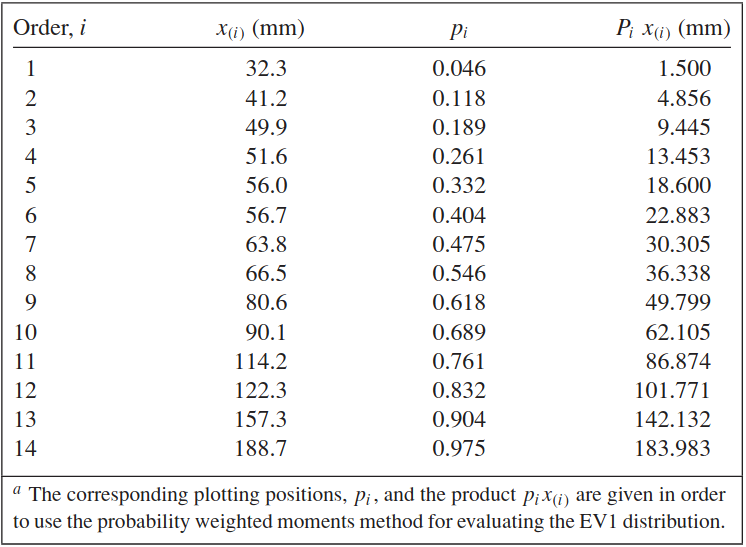
\includegraphics[width=\textwidth]{ta321.png}
\end{minipage}
 \hfill
\begin{minipage}{0.48\textwidth}
    Note that the values of $p_i$ correspond to \emph{plotting positions} for the ordered values $x_i$. According to the values in the table, $M_0 = 83.7$ mm and $M_1 = 54.6$ mm. The estimated values of $\hat{a}$ and $\hat{b}$ are:
    \[
        \hat{a} = \frac{2 M_1 - M_0}{\ln 2} = \frac{2 x 54.6 - 83.7}{\ln 2} = 36.8 \text{ mm} 
    \]

    \[
        \hat{b} = M_0 - a n_e = 83.7 - 36.8 x 0.5772 = 62.4 \text{ mm}
    \]

\end{minipage}

    \end{exampleblock}
\end{frame}

\begin{frame}{Estimation of parameters}
    \begin{exampleblock}{Extreme storms}
        The following figure shows the probability of exceedence ($Pr[X>x] = 1 - F_X (x)$) for the observed data, the theoretical extreme value distribution whose coefficients ($a$ y $b$) were estimated using the \emph{methods of moments} and the \emph{pwms}.  
    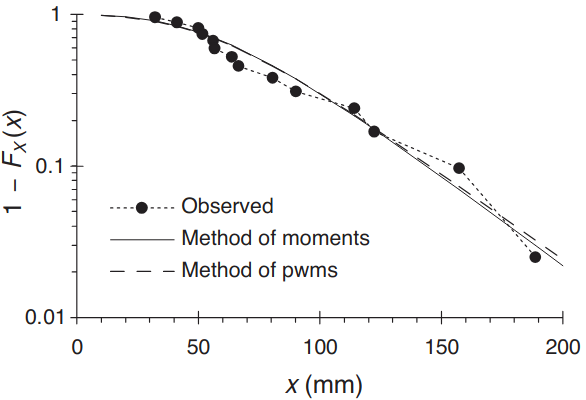
\includegraphics[width=\textwidth]{fi325.png}
    \end{exampleblock}
\end{frame}

\begin{frame}{Estimation of parameters}
    \begin{block}{Maximum likelihood method}
        For a given random variable $X$, a sample of size $n$ is taken from the  space space, and the \emph{pdf} is $f_X (x)$. The \alert{likelihood function} of $\theta$, where $\theta$ is vector of $m$ parameters, is represented as:
        \[
            L (\theta) = \prod_{i=1}^n f_X (x_i | \theta )
        \]
        The objective is to  find the vector $\theta$ that maximize $L(\theta)$ for a given $X$ sample. It is thus necessary to obtain the $m$ partial derivative of $L(\theta)$ with respect to each $\theta$ parameter. Derivatives are equated to zero and solved  to find the \alert{maximum likelihood (ML)} estimators ($\hat{\theta}$) of $\theta$.  
    \end{block}

    \begin{exampleblock}{Flood exeedance}
        Suppose that $X$ is a discrete random variable that determine the exceedance of a discharge threshold. Accordingly, $X$ is equal to 1 where $X > x_{threshold}$ (flood occurrence) and equal to zero where $X \leq x_{threshold}$ (no occurrence of flood, complementary event). After the analysis of gauge streamflow data, the probability of $X = 1$ is equal to $p$ and the probability of $X = 0$ is $(1-p)$. If the \emph{pmf} of $X$ is a \emph{Bernoulli distribution}:
        \[
            P_X (x_j) = Pr [X = x_j] = p^{x_j} (1-p)^{1-x_j}, \text{ for } x_j = 0, 1
        \]
        Note that $p$ is the parameter of the $pmf$. The \emph{likelihood function} for $n$ trials or outcomes is:
        \[
            L (p) = \prod_{j=1}^n p^{x_j} (1-p)^{1-x_j}, \text{ for } x_j = 0, 1
        \]
    \end{exampleblock}
\end{frame}

\begin{frame}{Estimation of parameters}
    \begin{exampleblock}{Flood exeedance}
        A fundamental identity indicate that $\ln \left( \prod_{i=1}^n a_i \right) = \sum_{i=1}^n \ln a_i$. Following this:
        \[
            \ln L (p) = \ln \left( \prod_{j=1}^n p^{x_j} (1-p)^{1-x_j} \right) = \sum_{j=1}^n \ln \left( p^{x_j} (1-p)^{1-x_j} \right) 
        \]
        Then:
        \[
            \ln L (p) = \ln p \sum_{j=1}^n x_j  +  \ln (1-p)\sum_{j=1}^n (1-x_j)
        \]
        The derivative is:
        \[
            \frac{d \left( L (p) \right)}{dp} = \frac{1}{p} \sum_{j=1}^n x_j - \frac{1}{1-p}\sum_{j=1}^n (1-x_j) = \frac{\sum_{j=1}^n x_j}{p} - \frac{n - \sum_{j=1}^n x_j}{1-p}
        \]
        Equaling to zero and solving for $p$:
        \[
            \hat{p} = \frac{\sum_{j=1}^n x_j}{n}
        \]
        where $\hat{p}$ is and estimator of $p$. 
    \end{exampleblock}
    The \emph{maximum likelihood method} is the most implemented method. However, large samples are required to prevent the estimator becomes unbiased. This estimator does not have a low variance in comparison with others. Sometimes the estimators can be obtained analytically so numerical methods are needed.
\end{frame}

\section{Multiple random variables} % From Kotte

\subsection{Joint probability distribution of discrete variables} % From Kotte
\begin{frame}{Multiple random variables}
    \begin{itemize}
        \item So far, only \emph{single random variables} have been considered belonging to a population.  
        \item To describe individual random variables, \emph{univariate distributions} have been considered.
        \item In these section, experiments where two or more random variables occur simultaneously are studied. 
        \item Variables are studied jointly and their distribution are of the multivariate type.
        \item For \emph{multiple variables}, probabilities laws are described by \emph{joint probability mass or density functions}.
        \item An example of a continuous bivariate distribution is given by the mean hourly wind speed and wind direction recorded by a weather station. Note that both random variables occurred simultaneously. 
    \end{itemize}
\end{frame}

\begin{frame}{Joint probability distribution of discrete variables}
    \begin{block}{Joint probability mass function}
        Given two discrete random variables $X$ y $Y$, the joint (bivariate) \alert{pmf} is given by the intersection probability $p_{X,Y} (x,y) = Pr[(X=x) \cap (Y=y)]$. According to the proability axioms, $\sum_{\text{all } x_i} \sum_{\text{all } y_j} p_{X,Y} (x_i, y_j) = 1$. The joint \alert{cdf} is given by $ F_{X,Y} (x,y) = Pr[(X\leq x) \cap (Y\leq y)] =\sum_{x_i\leq x} \sum_{y_j\leq y} p_{X,Y} (x_i, y_j)  $.
        For $n$ randon variables $X$, the joint \emph{pmf} is given by:
        \[
            \displaystyle
            p_{X_1, X_2, \cdots, X_n} = Pr[(X_1 = x_1) \cap (X_2 = x_2) \cap \cdots \cap (X_n = x_n)]
        \]
        and the joint \emph{cdf} is given by:
        \begin{align*}
            \displaystyle
            F_{X_1, X_2, \cdots, X_n} &= Pr[(X_1 \leq x_1) \cap (X_2 \leq x_2) \cap \cdots \cap (X_n \leq x_n)] \\
                                      &= \sum_{x_{1_i}\leq x_1}  \sum_{x_{2_j}\leq x_1} \cdots \sum_{x_{n_k}\leq x_n} p_{X_1, X_2, \cdots, X_n} (x_{1_i}, x_{2_j}, \cdots, x_{n_k})
        \end{align*}
    \end{block}

    \begin{exampleblock}{Wind records}
        In an urban area, two different weather stations, whose precisions are different, measure wind speed. Engineers are interested to measure the number of days per year that wind speed,  in each station, surpases an speed threshold.  As these winds are liable to cause infrastructure damages, for design purposes, it is needed to estimate the joint probability of the number of days per year where wind speed is $>$ 60 km/h estimated using the two instruments. The following table shows the \emph{pmf} for the variables measured at the accurate station $X$ and the less accurate station $Y$. 
        
    \end{exampleblock}
\end{frame}

\begin{frame}{Joint probability distribution of discrete variables}
    \begin{exampleblock}{Wind records}
         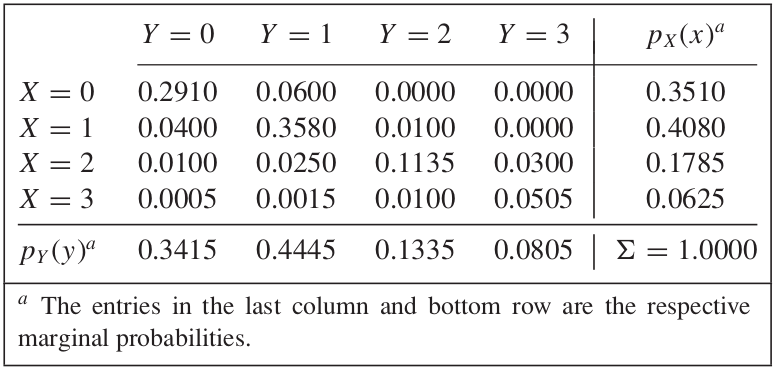
\includegraphics[width=\linewidth]{ta331.png}        
         Note that this table also show the \alert{marginal pmf} of $X$ and $Y$. Suppose that one want to judge the accuracy of $Y$, the probability that ($X=Y$) (event A) can be calculated as:
         \[
            \displaystyle
            Pr[A] = \sum_{\text{all } x_i} p_{X,Y} (x_i, y_i) = p_{X,Y} (0,0) + p_{X,Y} (1,1) + p_{X,Y} (2,2) + p_{X,Y} (3,3) = 0.813  
        \]
    \end{exampleblock}
\end{frame}
\begin{frame}{Joint probability distribution of discrete variables}
    \begin{block}{Conditional probability mass function}
        Given two discrete random variables $X$ and $Y$ whose joint \emph{pmf} is given by $p_{X,Y} (x,y)$, the \alert{conditional probability mass function} given that a value of $Y$ equal to $y_j$ is:
        \begin{align*}
            \displaystyle
            p_{X | Y} (x | y_j ) &= Pr[X = x | Y = y_j] = \frac{Pr[(X = x) \cap (Y = y_j)]}{Pr[Y = y_j]} \\ 
                                 &= \frac{p_{X,Y} (x, y_j)}{\sum_{\text{all } x_i} p_{X,Y}(x_i, y_j)} = \frac{p_{X,Y} (x, y_j)}{p_Y (y_j)} \quad \text{, for all $j$}
        \end{align*}
        Accorging to the probability axioms, $0 \leq p_{X,Y} (x | y_j) \leq 1, \quad \text{for all $j$}$ and $\sum_{\text{all } x_i} p_{X|Y} (x_i, y_j) = 1, \quad \text{for all $j$}$.
        Other conditional probability distribution are derived, for instance, when one wants to know the probability distribution of $X$ when $Y \geq y$. So:
         \[
            \displaystyle
            p_{X|Y \geq y} \equiv Pr[X = x| Y \geq y] = \frac{\sum_{y_j \geq y} p_{X,Y}(x, y_j)}{\sum_{y_j \geq y} p_{Y}(y_j)}
        \]
        Engineers are aware that almost all observed events are conditioned by the occurrence of other events. This is why, in practice, conditional probabilities are more easily obtained than joint \emph{pmf}s. Accordingly, the joint \emph{pmf} can be obtained using the conditional \emph{pmf} and the corresponding marginal \emph{pmf} as follows:
         \[
            \displaystyle
            p_{X,Y} (x,y) = p_{X|Y} (x|y)p_Y (y) = p_{Y|X} (y|x) p_X (x)
        \]
    \end{block}
\end{frame}

\begin{frame}{Joint probability distribution of discrete variables}
    \begin{exampleblock}{Wind records}
        According to the table above, if $Y = 1$, the joint probabilities $p_{X,Y} (x, 1)$  are given by 0.0600, 0.3580, 0.0250 and 0.0015 for $x = 0, 1, 2 \text{ and } 3$. The sum of these probabilities, $p_Y (Y=1) = 0.4445$. The conditional pmf, $p_{X|Y}(x|1)$ is given by 0.1350, 0.8054, 0.0562 and 0.0034, for $x = 0, 1, 2 \text{ and } 3$. Note that the sum of $p_{X|Y}(x|1)$ is 1.
    \end{exampleblock}

    \begin{block}{Marginal probability mass function}
        For multiples random variables, if all variables are disregarded apart from the single variable $X_i$, the \alert{marginal pmf} of $X_i$ can be obtained from the joint \emph{pmf}. For instance, for a bivariate joint \emph{pmf}, the marginal \emph{pmf} of $X$ (or for $Y$) is:
        \[
            \displaystyle
            p_X (x) \equiv Pr[X = x] = \sum_{\text{all } y_j} Pr[X=x | Y = y_j] Pr[Y= y_j] = \sum_{\text{all } y_j} p_{X,Y} (x, y_j)
        \]
        The \emph{cdf} can be obtained from this equation as follow:
        \[
            \displaystyle
            F_X (x) \equiv Pr[X \leq x] = \sum_{x_i \leq x} \sum_{\text{all } y_j}  p_{X,Y} (x_i, y_j)
        \]
   \end{block}
\end{frame}

\begin{frame}{Joint probability distribution of discrete variables}
     \begin{exampleblock}{Wind records}
         From the table of wind records, suppose that the engineer want to know the $Pr[X=0]$, so applying marginal \emph{pmf} equation  $p_X (0) = Pr[X = 0] = \sum_{y=0}^3 p_{X,Y}(0,y) = 0.2910 + 0.0600 + 0.0000 + 0.0000 = 0.3510$. The $Pr[X>0]$ can be obtained using the \emph{cdf} and is equal to 0.6490. The following figures show the marginal \emph{pmf} of $X$ and $Y$. 
\begin{minipage}[t]{0.49\textwidth}
\centering
         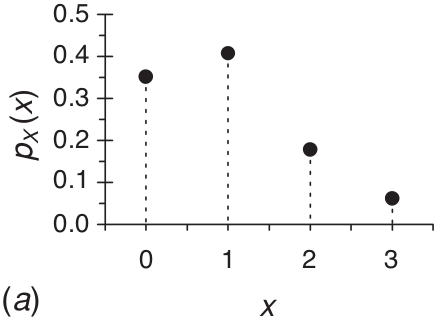
\includegraphics[width=0.6\linewidth]{fi331a.png}        
\end{minipage}
\hfill
\begin{minipage}[t]{0.49\textwidth}
\centering
         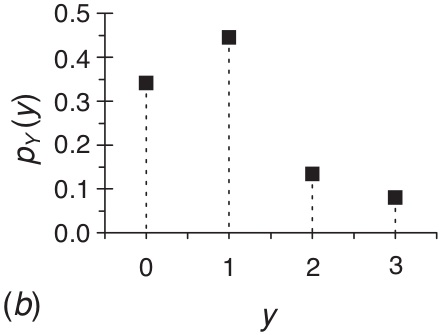
\includegraphics[width=0.6\linewidth]{fi331b.png}        
\end{minipage}
    \end{exampleblock}
    \begin{block}{Independent discrete random variable}
        If the events $X = x$ and $Y = y$ are statistically independent (or $X$ and $Y$ are statistically independent), the contidional \emph{pmf} is:
        \[
            \displaystyle
            p_{X|Y} (x|y) = p_X (x) \quad \text{and} \quad p_{Y|X} (y|x) = p_Y (y)
        \]
        and the joint \emph{pmf} is:
        \[
            \displaystyle
            p_{X,Y}(x,y) = p_X (x) p_Y (y)
        \]
   \end{block}
\end{frame}
\subsection{Joint probability distribution of continuous variables} % From Kotte

\begin{frame}{Joint probability distribution of continuous variables}

    \begin{block}{Joint pdf and cdf for continuos $X$ and $Y$ variables}
        If two continuos random variables $X$ and $Y$ ocurr simultaneously or are related somehow, the joint probability distribution is described by the \alert{joint probability density function} (\emph{pdf}), $f_{X,Y} (x,y)$. The probability over a region of interest $\{(x_1, x_2), (y_1, y_2)\}$, where $x_1 < x_2$ and $y_1 < y_2$, is defined as:
        \[
            \displaystyle
            Pr[(x_1\leq X \leq x_2) \cap (y_1\leq Y \leq y_2)] = \int_{x_1}^{x_2} \int_{y_1}^{y_2} f_{X,Y} (x,y) dy dx
        \]

\begin{minipage}{0.49\textwidth}
        As shown in the figure, this integral represent the volume below the surface represented by the joint \emph{pdf} over the region of interest. 
        According to the probability axioms, the $f_{X,Y} (x,y)$ has the following properties:
        \[
            \displaystyle
            f_{X,Y} (x, y) \geq 0
        \]
        \[
            \displaystyle
        \int_{-\infty}^{\infty} \int_{-\infty}^{\infty} f_{X,Y} (x,y) dy dx = 1
        \]
\end{minipage}
%\hfill
\begin{minipage}{0.49\textwidth}
    
%\centering
         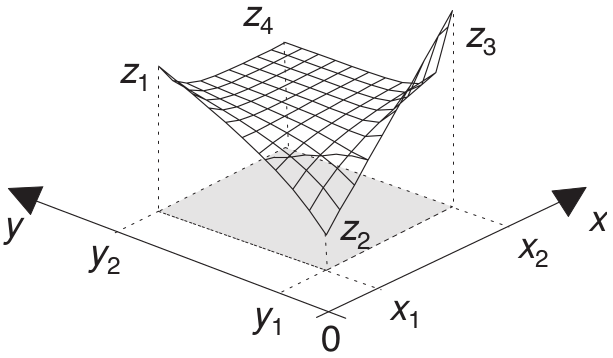
\includegraphics[width=\linewidth]{fi333.png}        

\end{minipage}
The \alert{joint cumulative distribution function} (\emph{cdf}), $F_{X,Y} (x,y)$, is defined as:
        \[
            \displaystyle
            F_{X,Y} (x,y) \equiv Pr[(-\infty \leq X \leq x) \cap (\infty \leq Y \leq y)] = \int_{-\infty}^{x} \int_{-\infty}^{y} f_{X,Y} (x,y) dy dx
        \]

   \end{block}
\end{frame}

\begin{frame}{Joint probability distribution of continuous variables}

    \begin{block}{Joint pdf and cdf for continuos $X$ and $Y$ variables}
        These concepts can be applied to $n$ random variables $X$ defined on the same probability space. So $(X_1, X_2, \cdots, X_n)$ is an \alert{n-dimensional continuous random variable } if $f_{X_1, X_2, \cdots, X_n} (x_1, x_2, \cdots, x_n) \geq 0$. Accordingly:
        \begin{align*}
            \displaystyle
            &F_{X_1, X_2, \cdots, X_n} (x_1, x_2, \cdots, x_n) \\
            &\equiv Pr[(-\infty \leq X_1 \leq x_1) \cap (\infty \leq X_2 \leq x_2) \cap \cdots \cap (\infty \leq X_n \leq x_n)] \\
            &= \int_{-\infty}^{x_1} \int_{-\infty}^{x_2} \cdots \int_{-\infty}^{x_n} f_{X_1, X_2, \cdots, X_n} (x_1, x_2, \cdots, x_n) dx_1 dx_2 \cdots dx_n
        \end{align*}
        where $(x_1, x_2, \cdots, x_n)$ is a \emph{n-tuple} of points in the sample space. 
        Recalling from the univariate case, the \emph{pdf} and the \emph{cdf} are related for the bivariate case as:
\[
            \displaystyle
            f_{X,Y} (x,y) = \frac{\partial^2 }{\partial x \partial y} F_{X,Y} (x,y)
        \]
        For $n$ random variables:
\[
            \displaystyle
             f_{X_1, X_2, \cdots, X_n} (x_1, x_2, \cdots, x_n) = \frac{\partial^n }{\partial x_1 \partial x_2  \cdots \partial x_n}F_{X_1, X_2, \cdots, X_n} (x_1, x_2, \cdots, x_n)
        \]

   \end{block}
\end{frame}

\begin{frame}{Joint probability distribution of continuous variables}

    \begin{exampleblock}{Storm intensity and duration}
        An storm occurring in place on earth is characterized its \emph{intensity} and its \emph{duration}, where the intensity is the average amount of rain fell. Suppose that intensity and duration are two continuous random variables, $Y$ and $X$, respectively. It is known that the \emph{cdf} of $X$ and $Y$ are represented by:
        \[
            F_X (x) = 1 - e^{-ax},\ x \geq 0, a >0; \quad F_Y (y) = 1 - e^{-by},\ y \geq 0, b >0; 
        \]
        where $a$ and $b$ are parameters of the \emph{cdf}s. Accordingly, it is assumed that the joint \emph{cdf} is given by the exponential bivariate distribution:
        \[
            F_{X,Y} (x,y) = 1 - e^{-ax} - e^{-by}+e^{-ax-by-cxy}
        \]
        where $c$ is a parameter of the joint \emph{cdf} that describes the joint variability (or correlation) of $X$ and $Y$ . According to the marginal \emph{cdf}s, $a$ and $b$ are $>$ 0, so that, one might be interested to known the possible values of $c$. To search for the lower bound of $c$, it is known by definition that $F_{X,Y} (x,y) \leq F_X (x)$, because the joint $Pr[X\leq x, Y\leq y]$ can not exceed $Pr[X\leq x]$ independently of the value taken by $Y$. The same apply for $Y$. Accordingly:
        \vspace{-5pt}
        \[
            F_{X,Y} (x,y) = 1 - e^{-ax} - e^{-by}+e^{-ax-by-cxy} \leq F_X (x) = 1 - e^{-ax}
        \]
        resolving:
        \vspace{-5pt}
        \begin{align*}
            -e^{-by}-e^{-ax-by-cxy} \leq 0 \quad e^{-ax-by-cxy} \leq e^{-by} \quad -x(a+cy) \leq 0
        \end{align*}
        Regarding that $X$ and $Y$ are non negative variables, the inequality $-x(a +cy)\leq 0$ holds if and only if $(a+cy)\geq 0$. 

    \end{exampleblock}
\end{frame}


\begin{frame}{Joint probability distribution of continuous variables}
    \begin{exampleblock}{Storm intensity and duration}
To determine the upper bound of $c$ we need to get the joint \emph{pdf}. So that, first we get the partial derivative with respect to $x$ and then with respect to $y$: 
\[
    \frac{\partial F}{\partial x} = \frac{\partial \left(1-e^{-ax}-e^{-by}+e^{-ax-by-cxy} \right)}{\partial x} = a e^{-ax} - (a + cy)e^{-ax-by-cxy}
\]

        \begin{align*}
            f_{X,Y}(x,y) &= \frac{\partial^2 F}{\partial x \partial y} = \frac{\partial \left( a e^{-ax} - (a + cy)e^{-ax-by-cxy}\right)}{\partial y} \\
                         &= \left[ (a+cy)(b+cx)-c \right]e^{-ax-by-cxy}
        \end{align*}
        Accordingly, the for $x=y=0$, $f_{X,Y}(0,0)= ab-c$. Since the joint \emph{pdf} is a non-negative function, the inequality $ab-c \geq 0$ must hold, so the upper bound of $c$ is $c\leq ab$. Summing up, the bivariate exponential distribution is defined for $0 \leq c \leq ab$. 
    \end{exampleblock}
\end{frame}

\begin{frame}{Joint probability distribution of continuous variables}
    \begin{block}{Conditional probability density function}

        The \alert{conditional density function} of $Y$ given $X$ is written as:
        \[
        f_{Y | X} (y|x) = \frac{f_{X,Y} (x,y)}{f_X (x)}
    \]
    From where,
        \[
         f_{X,Y} (x,y)=f_{Y | X} (y|x) f_X (x) = f_{X | Y} (x|y) f_Y (y)
    \]

    \end{block}
    \begin{exampleblock}{Storm intensity and duration}
        From the example above, it is known that $a>0$, $b>0$ and $0\leq c \leq 1$ are three parameters estimated based on rainfall data. For weather station, the following values were estimated: $a =$ 0.05 h$^{-1}$, $b =$ 1.2 h/mm and $c = $ 0.06 mm$^{-1}$. Engineers are planning to design a drainage system, so they need to estimate the probability that an storm lasting $X =$ 6 hours will exceed an average intensity of $Y = $ 2 mm/h.
        The conditional \emph{pdf} of the storm intensity for a given duration is:
        \begin{align*}
            f_{Y|X} (y|x) &= \frac{f_{X,Y (x,y)}}{f_X(x)} = \frac{\left[ (a+cy)(b+cx)-c \right]e^{-ax-by-cxy}}{a e^{-ax}} \\
                          &= a^{-1}\left[ (a+cy)(b+cx)-c \right]e^{-y(b+cx)}
        \end{align*}

    \end{exampleblock}
\end{frame}

\begin{frame}{Joint probability distribution of continuous variables}
    \begin{exampleblock}{Storm intensity and duration}
        The conditional cdf is (making $y \equiv u$):
         \begin{align*}
             \displaystyle
             F_{Y|X} (y|x) &= \int_0^y a^{-1}\left[ (a+cu)(b+cx)-c \right]e^{-u(b+cx)} du\\
            &= a^{-1}(b+cx)\int_0^y (a + cu)e^{-u(b+cx)}du -a^{-1} c \int_0^y  e^{-u(b+cx)}du \\
            &= 1-\frac{a+cy}{a}e^{-y(b+cx)}
        \end{align*}
        Evaluating the following:
\[
    Pr[Y> 2 | X=6] = 1- F_{Y|X} (2|6) = 1 - 1 + \frac{0.05 + 0.06 x 2}{0.05} e^{-2(1.2+0.06 x 6)} = 0.15
\]
    \end{exampleblock}
\end{frame}

\begin{frame}{Joint probability distribution of continuous variables}
    \begin{block}{Independent continuous random variable}
        If the events $X=x$ and $Y=y$ are stochastically independent, then $f_{X|Y} (x,y) = f_X (x)$ and $f_{Y|X} (y,x) = f_Y (y)$, therefore $f_{X,Y} (x,y) = f_X (x) f_Y (y)$. 
        Note that the assumption of independence simplifies the application of probability to engineering problems. 
    \end{block}
    
    \begin{exampleblock}{Storm intensity and duration}
        If the joint variability of storm duration  $X$ and storm intensity $Y$, is neglected, the joint \emph{pdf} is given by:
        \[
            f_{X,Y} (x,y) = f_X (x) f_Y (y) = a e^{-ax} b e^{-by} = ab \ e^{-ax-by}
        \]
        The same expression is valid for $c=0$.
    \end{exampleblock}
    \begin{block}{Marginal probability density function}
        The extension of the \emph{total probability theorem} gives:
        \[
            \displaystyle
            f_X (x) = \int_{-\infty}^{\infty} f_{X|Y} (x|y) f_Y (y) dy = \int_{-\infty}^{\infty} f_{X,Y} (x,y) dy
        \]

        \[
            \displaystyle
            f_Y (y) = \int_{-\infty}^{\infty} f_{Y|X} (y|x) f_X (x) dx = \int_{-\infty}^{\infty} f_{X,Y} (x,y) dx
        \]
    \end{block}
\end{frame}


\begin{frame}{Joint probability distribution of continuous variables}
    \begin{exampleblock}{Storm intensity and duration}
        The joint \emph{pdf} for the storm duration $X$ and the storm intensity $Y$ is $f_{X,Y} (x,y) = \left[ (a+cy)(b+cx)-c \right]e^{-ax-by-cxy}$. From the definition of marginal probability density function:
\[
            \displaystyle
            f_X (x) =  \int_{0}^{\infty} f_{X,Y} (x,y) dy = \int_{0}^{\infty} \left[ (a+cy)(b+cx)-c \right]e^{-ax-by-cxy} dy  = a \ e^{-ax}
        \]

\[
            \displaystyle
            f_Y (y) =  \int_{0}^{\infty} f_{X,Y} (x,y) dx = \int_{0}^{\infty} \left[ (a+cy)(b+cx)-c \right]e^{-ax-by-cxy} dx = b \ e^{-by}
        \]

    \end{exampleblock}
\end{frame}

\subsection{Properties of multiple variables} % From Kotte

\begin{frame}{Properties of multiple variables}

    \begin{block}{Covariance and correlation}
        The \emph{expectation operator (E)} introduced in below for a single variable can be used on two or more random variables. For instance, for the linear combination of two random variables $X_1$ and $X_2$, $E[a X_1 + b X_2 ] = aE[X_1 ]+bE[X_2 ]$, where $a$ and $b$ are constants. Accordingly, the variance of $aX_1 + bX_2$ is:
        \[
            Var[aX_1 + bX_2] = a^2 Var[X_1] + b^2 Var[X_2]- 2ab Cov[X_1 , X_2]
        \]
        where the operator $Var$ is the variance operator and $Cov$ is the \alert{covariance} operator. The \alert{covariance} of $X_1$ and $X_2$ is calculated as:
        \[
            Cov[X_1 , X_2 ] = E[(X_1 - E[X_1]) (X_2 - E[X_2])] = E[X_1 X_2]-E[X_1] E[X_2] 
        \]
        where $ E[X_1 X_2] = \int_{-\infty}^{\infty} \int_{-\infty}^{\infty} x_1 x_2 f_{X_1 , X_2} (x_1, x_2) d_{x_1} d_{x_2}$. If $X_1$ and $X_2$ are independent:
         \begin{align*}
             E[X_1 X_2] &= \int_{-\infty}^{\infty} \int_{-\infty}^{\infty} x_1 x_2 f_{X_1 , X_2} (x_1, x_2) d_{x_1} d_{x_2} \\
                        &=\left[ \int_{-\infty}^{\infty} x_1 f_{X_1} (x_1) dx_1 \right]\left[ \int_{-\infty}^{\infty} x_2 f_{X_2} (x_2) dx_2 \right] \\
                        &= E[X_1] E[X_2]
        \end{align*}
        therefore $Cov[X_1 , X_2 ] = 0$ and $Var[aX_1 + bX_2] = a^2 Var[X_1] + b^2 Var[X_2]$. 
    \end{block}

\end{frame}

\begin{frame}{Properties of multiple variables}
    \begin{exampleblock}{Storm intensity and duration}
        The joint \emph{pdf} of the independent random variables, storm duration $X$ and storm intensity $Y$, is $f_{X,Y} (x,y)= f_X (x) f_Y (y) = a \ e^{-ax} b \ e^{-by} = ab \ e^{-ax-by}$, where $\mu_X = a^{-1}$ and $\mu_Y = b^{-1}$. To estimate $Cov[X,Y]$, it is needed to estimated:
        \[
            E[XY] = \int_{0}^{\infty} \int_{0}^{\infty} xy f_{X,Y} (x,y) dx dy = \int_{0}^{\infty} \int_{0}^{\infty} xy \ ab \ e^{-ax - by} dx dy = \frac{1}{ab}
        \]
        The $Cov[X,Y]$ is:
        \[
            Cov[X,Y] = E[XY] - E[X] E[Y] = \frac{1}{ab} - \frac{1}{a}\frac{1}{b} = 0
        \]

        This confirm that there is no covariance between $X$ and $Y$.
    \end{exampleblock}
    \begin{block}{Coefficient of linear correlation}
    Note that $Cov[X_1,X_2]$ is positive and large when both variables are large or small with respect to their means.In contrast,  $Cov[X_1,X_2]$ can be negative and large when both variables are equidistand (e.g. one small and the other large). Note that covariance is a mesuare of the linear relationship between variables; no linearly related variables yield no covariance. The linear relationship between $X_1$ and $X_2$ is defined as the \alert{coefficient of linear correlation ($\rho$)}:
    \[
        \rho = \frac{Cov[X_1, X_2]}{\sigma_{X_1} \sigma_{X_2}}
    \]
    where $-1 \leq \rho \leq 1$.
        \end{block}
\end{frame}


\begin{frame}{Properties of multiple variables}
    \begin{block}{Joint moment-generating function}
        The \alert{Joint moment-generating function} for multiple random variables $X_1, X_2, \cdots, X_k$ is:
        \[
            M_{X_1, X_2, \cdots, X_k} (t_1, t_2, \cdots, t_k) = E\left[ e^{\left( \sum_{i=1}^k t_i X_i \right)}\right] 
    \]
    where the $rth$ moment of $X_i$ can be computed by diferentiating the joint moment-generating function $r$ times with respect to $t_i$ and then evaluating the derivative for $t_i = 0$. 
    For two statistically independent random variables, $X_1$ and $X_2$, the \emph{Joint moment-generating function} is:
    \[
        M_{X_1, X_2} (t_1, t_2) = E[e^{t_1 X_1 + t_2 X_2}] = E[e^{t_1 X_1}] E[ e^{t_2 X_2} ] = M_{X_1} (t_1) M_{X_2} (t_2)
    \]
    This means that if the joint \emph{mgf} of two variables equal the product of individual \emph{mgf}s, the two variables are statistically independent. 
        \end{block}

    \begin{exampleblock}{Storm intensity and duration}
        The joint \emph{pdf} of the independent random variables, storm duration $X$ and storm intensity $Y$, is $f_{X,Y} (x,y) = ab \ e^{-ax-by}$, where $\mu_X = a^{-1}$ and $\mu_Y = b^{-1}$. The joint \emph{mgf} of $X$ and $Y$ is:
        \[
            M_{X,Y} (t_1, t_2) = E \left[ e^{t_1 X + t_2 Y} \right] = E \left[ e^{t_1 X} \right] E \left[ e^{t_2 Y} \right] = \frac{ab}{(a-t_1) (b-t_2)}
        \]

    \end{exampleblock}
\end{frame}

% Other topic not included
%%  3.4 ASSOCIATED RANDOM VARIABLES AND PROBABILITIES Kotte
%%  3.5 COPULAS Kotte

\section{Probability distributions} % From Diaz-G

\begin{frame}{Probability distributions}
    \begin{block}{Generalities}
        \begin{itemize}
            \item From the data sample representation is possible to obtain the \alert{empirical distribution}. 
            \item The \alert{probability distributions} are mathematical functions that satisfy the probability axioms. 
            \item These distributions or functions are appropriate to describe analytically the random behaviour of certain variables and are interpreted as probability models. 
            \item Accordingly, the probability distributions establish the probability of occurrence of a value taken by the random variable. 
            \item A random variable can be represented by multiple distributions, however the \''closest one\'' to the empirical distribution  must be chosen. 
            \item In hydrology, there are certain distributions that adjust the best to some hydrological variables according to decades of experience. 
            \item To fit a probability distribution to a random variable upon a random variable sample is needed to adjust the distribution \alert{parameters}.
            \item The more parameters the function has, the most flexible is the distribution to fit the empirical distribution. However the more parameters, the less degrees of freedom.
            \item Probability distributions can according to the random variable type:
                \begin{itemize}
                    \item Discrete probability distributions: Used for discrete random variables
                    \item Continuous probability distributions: Used for continuous random variables
                \end{itemize}
        \end{itemize}
    \end{block}

\end{frame}
\subsection{Discrete probability distributions} % From Diaz-G, Ben and Cornell and Kotte
% WARNING! THIS SUBSECTION NEEDS TO BE UPDATED BASED ON THE HANDNOTES
\begin{frame}{Discrete probability distributions}

    \begin{block}{The \alert{binomial} distribution}
        This distribution is used to define the probabilities of discrete random variables. For a sample of size $n$ an instance of the random variable only take two values (0 or 1, success or failure). The $n$ observations or experiments are mutually exclusive and collectively exhaustive, and the probability of occurrence of either value is constant. Each observation or experiment follow a \alert{Bernoulli distribution} where the probability of success is $p$ and the probability of failure is $1-p$. The set of $n$ observations or experiments is known as the experiments of Bernoulli from where a random variable $X$, which represents the observation with success in $n$ observations, follows a \alert{Binomial distribution}:
        \[
            p_X (x) = Pr[X = x; n,p] = B(x;n,p) = \binom{n}{x} p^x (1-p)^{n-x}
        \]
        where $n$ and $p$ are parameters of the distribution, $x=0,1,\cdots, n$, $0 \leq p \leq 1$ and $\binom{n}{k}=\frac{n!}{x! (n-x)!}$; this term represents the possible combinations to obtain $x$ success from $n$. The \emph{cmf} is:
        \[
            F_X (x) = Pr[X\leq x] = \sum_{k=0}^x \binom{n}{k} p^k (1-p)^{n-k}
        \]
        For this distribution, the mean is $E[X] = np$ and the variance is $Var[X] = np(1-p)$.
    \end{block}
    \end{frame}

\begin{frame}{Discrete probability distributions}
\begin{exampleblock}{Flooding of a road} % From Kotte
        The probability that a road is flooded once in a give year is $p=0.1$. Compute the probability that the road will be flooded at least once during a five-year period. So the $Pr[X \geq 1] = Pr[X = 1;5,0.1] + Pr[X=2;5,0.1] + Pr[X=3;5,0.1]+ Pr[X=4;5,0.1] + Pr[X=5;5,0.1] = 0.3281 + 0.0729 + 0.0081 + 0.0005 + 0.00001 = 0.4095$. An alternative to  estimate this probability is to determine the probability of no flooded during the period ($Pr[X < 1]= 1-Pr[X \geq 1]$). So $Pr[X \geq 1] = 1-Pr[X=0;5,0.1] = 1-0.5905 = 0.4095$. Note that in reality, the values of $p$ can change year to year so the application of this model can be inaccurate. 
    \end{exampleblock}

    \begin{block}{The \alert{geometric} distribution}
        This distribution characterizes the probability of a random variable $X$ that represents the Bernoulli's trials upon one get a success. So:
        \[
            P_X (x) = Pr[X = x; p] = (1-p)^{x-1} p
        \]
        where $p$ ($0 < p \leq 1$) is the probability of success in the Bernoulli's trials, and $X = 0,1,2, \cdots$, $x-1$ failures before the first success. A converging \emph{geometric series} $\sum_{x=1}^{\infty} (1-p)^x = \frac{1-p}{p}$. To optain the mean, one can derive both sides of the geometric series with respect to $p$ and multiply by $-p$, which is equivalent to $E[X] = \sum_{x=1}^\infty x (1-p)^{x-1} p = \frac{1}{p}$. To obtain $Var (X) = E[X(X-1)] = E[X^2] - E[X] = \sum_{x=1}^\infty x(x-1) (1-p)^{x-1} p = 
$
    \end{block}
\end{frame}

\begin{frame}{Discrete probability distributions}
    \begin{block}{The \alert{geometric} distribution}
        To obtain $Var (X)$ one use the second factorial moment as $E[X(X-1)] = E[X^2] - E[X] = \sum_{x=1}^\infty x(x-1) (1-p)^{x-1} p$. Getting the second derivative of the \emph{geometric series} with respect to $p$ and multiplying both sides by $p(1-p)$, one get that $E[X^2] - E[X] = \frac{2(1-p)}{p^2}$. Regarding this and that $Var (X) = E[X^2] - \left(E[X]\right)^2 = \frac{2(1-p)}{p^2}+ E[X]-\left(E[X]\right)^2 = \frac{2(1-p)}{p^2} + \frac{1}{p}- \frac{1}{p^2} = \frac{1-p}{p^2}$ 
    \end{block}
\end{frame}



\subsection{Continuous probability distributions} %% From Diaz-G, Ben and Cornell and Kotte
\begin{frame}{Continuous probability distributions}
    \emph{Continuous probability distributions} are applicable when the random variable is continuous; take any value in its real domain, e.g. river flow, air temperature. 
    \begin{block}{\alert{Uniform} distribution}
        It is the simplest distribution, and as it is indicated by its name, the \emph{pdf} is constant over a defined interval $a \leq x \leq b$. The \emph{pdf} is:
         \begin{align*}
             \displaystyle
             f_X (x) &= \frac{1}{b-a} \text{, for } a\leq x \leq \\
                     &= 0 \text{, otherwise}
        \end{align*}
        This distribution is also knows as the \emph{rectangular distribution}. Note that all values between $a$ and $b$ are equally probable and the area under the \emph{pdf} is equal to 1. The probability that $X$ fall in $(c,d)$ is $Pr[c < X < d] = \frac{d-c}{b-a}$. The unit uniform distribution is obtained when $a=0$ and $b=1$ ans it is commonly used to generate random variables in simulations. 
    \end{block}
\begin{minipage}{0.49\textwidth}
\centering
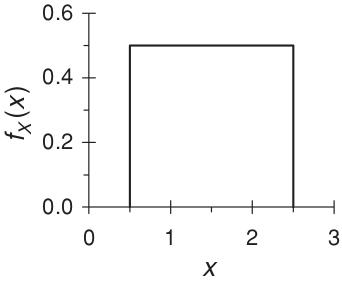
\includegraphics[width=0.8\linewidth]{fi421.png}  % from Kotte      
\end{minipage}
\hfill
\begin{minipage}{0.49\textwidth}
\centering
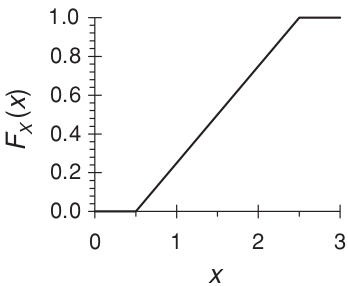
\includegraphics[width=0.8\linewidth]{fi422.png} % from Kotte
\end{minipage}

\end{frame}

\begin{frame}{Continuous probability distributions}
    \begin{block}{\alert{Uniform} distribution}

        \begin{itemize}
            \item \emph{Mean}
                \[
                    E[X] = \int_a^b \frac{x}{b-a} dx = \frac{1}{b-a} \left[ \frac{x^2}{2} \right]_a^b = \frac{b+a}{2}
                \]
            \item \emph{Variance}
         \begin{align*}
             \displaystyle
             Var[X] = E[X^2] - \left( E[X] \right)^2 &= \int_a^b \frac{x^2}{b-a} dx - \left( E[X] \right)^2  \\
                                                     &= \frac{1}{b-a} \left[ \frac{x^3}{3} \right]_a^b -  \frac{(b+a)^2}{4} \\
                                                     &= \frac{b^3 - a^3}{3(b-a)} - \frac{(b+a)^2}{4} = \frac{b^2 + ba + a^2}{3} - \frac{(b+a)^2}{4}\\
                                                     &= \frac{(b-a)^2}{12}
        \end{align*}
    \item \emph{Moment-generating function}
\[
    M_X (t) = E \left[e^{tX} \right] = \int_a^b \frac{e^{tx}}{b-a} dx = \frac{e^{tb} - e^{ta}}{t(b-a)}
\]

        \end{itemize}
    \end{block}
\end{frame}

\begin{frame}{Continuous probability distributions}
    \begin{block}{\alert{Exponential} distribution}
        From the \alert{Poisson process} discussed previously, if we denote by random variable $T$ the time to the first arrival, then the probability that $T$ exceeds some value $t$ is equal to the probability that no events occur in that time interval of length $t$. While former probability is 1 - $F_T (t)$, the latter probability $p_X (0)$ is zero, which is the probability that a Poisson random variable $X$ with parameter $\lambda t$. Replacing:
        \[
            1- F_T (t) = \frac{(\lambda t)^0 e^{-\lambda t}}{0!} = e^{-\lambda t} \quad t\geq 0
        \]
        Therefore:
        \[
            F_T (t) = 1 - e^{-\lambda t} \quad t\geq 0
        \]
        and the $f_t (t)$ is:
        \[
            f_T (t) = \frac{d F_T (t) }{dt} = \lambda e^{-\lambda t} \quad t\geq 0
        \]
        This equation define the \alert{exponential distribution}, which describes the time to the first occurence of a Poisson event. Note that $e^{-\lambda t}$ is the probability of no events in any interval of time of length $t$, whether or not it begins at time 0. In short, the interarrival times of a \alert{Poisson process} are independent and exponentially distributed. 
        \begin{itemize}
            \item \emph{Mean}
                \vspace{-5pt}
                \[
                    E[T] = \int_0^\infty t \lambda e^{-\lambda t} dt
                \]
                \vspace{-5pt}
                making $u=\lambda t$:
                \vspace{-5pt}
                \[
                    E[T] = \frac{1}{\lambda} \int_0^\infty u e^{-u} du = \frac{1}{\lambda} \left[ e^{-u} (-u-1) \right]_0^\infty = \frac{1}{\lambda}
                \]
        \end{itemize}
    \end{block}
\end{frame}

\begin{frame}{Continuous probability distributions}
    \begin{block}{\alert{Exponential} distribution}
                Note that if $\lambda$ is the rate at which events occur in a \emph{Poisson process}, $\frac{1}{\lambda}$ is the average time between events. 
       \begin{itemize}
            \item \emph{Variance}
                \vspace{-5pt}
         \begin{align*}
             \displaystyle
             Var[T] = E[T^2] - \left( E[T] \right)^2 &= \int_0^\infty t^2 \lambda e^{-\lambda t} dt - \left( E[X] \right)^2  \\
                                                     &= \frac{1}{\lambda^2} \int_0^\infty u^2 e^{-u} du - \frac{1}{\lambda^2} = \frac{1}{\lambda^2}
         \end{align*}
                \vspace{-5pt}
         It easy to show that  the \emph{coefficient of variation} $V_T = \frac{\sqrt{Var[T]}}{E[T]} = 1$.

    \item \emph{Moment-generating function}
                \vspace{-5pt}
\[
    M_X (t) = E \left[e^{tX} \right] = \int_0^\infty e^{tx} \lambda e^{-\lambda x} dx = \frac{\lambda}{\lambda - t}, \quad \text{for } t < \lambda 
\]
       \end{itemize}
    \end{block}
                \vspace{-10pt}
     \begin{exampleblock}{Floods affecting construction}
         Engineers are concerned of the occurrence of a flood exceeding 100 m$^3$ s$^{-1}$ that can seriously affect infrastructure. If this streamflow is exceeded once every five years on average based on historical flow records, what is the change that the infrastructure construction which is scheduled to last 14 months can proceed without interruptions or detrimental effects? 
         Suppose that flow exceeding this magnitude are independent and identically distributed events. The sample mean is $\bar{t} = 5$ years, thus $\bar{\lambda} = \frac{1}{5}$. From the exponential distribution, $Pr \left[ X \geq \frac{14}{12} \right] = e^{-1/5 . 14/12} = 0.79$. Accordingly, the risk is thus 1-0.79 = 0.21, which is quite high. The solution would be to shorten the period of construction. 
    \end{exampleblock}
\end{frame}

\begin{frame}{Continuous probability distributions}
    \begin{block}{\alert{Exponential} distribution}
        \begin{itemize}
            \item \emph{Memoryless property}
                The \emph{Poisson process} is often said to be \emph{memoryless} meaning that  future behaviour is independent of its present or past behaviour. This memoryless trait of the Poisson arrivals and of the exponential distribution is best understood by determining the conditional distribution of $T$ given that $T > t_0$, that is, the distribution of the time between arrivals given that no arrivals occurred before $t_0$:
                \vspace{-10pt}
                \[
                    F_{T|[T > t_0 ]} (t) = P[T \leq t | T > t_0] = \frac{P\left[(T \leq t) \cap (T > t_0) \right]}{P[T > t_0]}
                \]
                For $t < t_0$, the numerator is zero; for $t \geq t_0$ it is simply equal to $P[t_0 < T \leq t]$. Thus:
                \vspace{-5pt}
         \begin{align*}
             \displaystyle
             F_{T|[T > t_0 ]} (t) = \frac{F_T (t) - F_T (t_0)}{1- F_T (t_0)} &= \frac{(1-e^{-\lambda t}) - (1-e^{-\lambda t_0})}{e^{-\lambda t_0}} \\
                                                                             &= \frac{e^{-\lambda t_0}-e^{-\lambda t}}{e^{-\lambda t_0}} = 1-e^{-\lambda(t-t_0)} \quad t \geq t_0
         \end{align*}
         \[
             f_{T|[T> t_0]} (t) = \lambda e^{-\lambda (t-t_0)} \quad t \geq t_0
         \]
         If $\tau = t - t_0$, 
                \vspace{-5pt}
         \[
             f_{T|[T> t_0]} (t_0 + \tau) = \lambda e^{-\lambda \tau} \quad \tau \geq 0
         \]
          This means that failure to observe an event up to $t_0$ does not alter one's prediction of the length of time (from $t_0$) before an event will occur. The future is not influenced by the past if events are \emph{Poisson arrivals}. An implication is that any choice of the time origin is satisfactory for the \emph{Poisson process}.

        \end{itemize}
        
    \end{block}
\end{frame}

\begin{frame}{Continuous probability distributions} % From Diaz-Gra
    \begin{block}{\alert{Triangular} distribution}
        This distribution is defined in the range of $a \leq X \leq b$ and the \emph{pdf} is:
\[
f_X (x) =
\begin{cases}
    \frac{2(x-a)}{(b-a)(c-a)} & \text{if } a \leq x \leq c \\
    \frac{2(b-x)}{(b-a)(b-c)} & \text{if } c < x \leq b \\
    0 & \text{otherwise }
\end{cases}
\]
Note that $c$ correspond to the highest triangle vertex and it is the mode of \emph{pdf}. The \emph{cdf} is thus:
\[
F_X (x) =
\begin{cases}
    0 & \text{if } x < a \\
    \frac{(x-a)^2}{(b-a)(c-a)} & \text{if } a \leq x \leq c \\
    1-\frac{(b-x)^2}{(b-a)(b-c)} & \text{if } c < x \leq b \\
    1 & \text{otherwise }
\end{cases}
\]
\begin{itemize}
    \item \emph{Mean}
                \vspace{-5pt}
        \[
            E[X] = \int_a^b x f_X(x) dx = \frac{a+b+c}{3}
        \]
    \item \emph{Varianza}
                \vspace{-5pt}
        \[
            Var[X] = E[X^2] - \left( E[X] \right)^2 = \int_a^b x^2 f_X(x) dx - \left( E[X] \right)^2 = \frac{a^2 + b^2 + c^2 -ab-ac-bc}{18}
    \]
\end{itemize}
This distribution is used in hydrology as an alternative to the \alert{uniform distribution} to describe the sample space and the uncertainty of parameters in hydrological modelling. 

    \end{block}
\end{frame}

\begin{frame}{Continuous probability distributions} 
    \begin{block}{The \alert{Gamma} distribution}
        As in the case with discrete trials, it is also of interest to ask for the distribution of the time $X_k$ to the kth arrival of a \alert{Poisson process}. Now, the times between arrivals, $T_i$, $i= 1,2, \cdots, k$, are independent and have an exponential distribution with common parameter $\lambda$. $X_k$ is the sum  $T_1 + T_2 + \cdots + T_k$. Its distribution follows from repeated application of the convolution integral $f_Z (z) = \int_\infty^\infty f_X (z - y) f_Y (y) dy$, where $Z = X + Y$ and $X$ and $Y$ are independent. For any $k = 1, 2, 3, \cdots$:
        \[
            f_{X_k} (x) = \frac{\lambda (\lambda x)^{k-1} e^{-\lambda x}}{(k-1)!} \quad x \geq 0
        \]
        Thus, we say that $X$ follow a \emph{Gamma distribution} with parameters $k$ and $\lambda$. Regarding that $X$ can be considered as the sum of $k$ independent exponentially distributed random variables, then:
        \begin{itemize}
            \item \emph{Mean}
                \[
                    E[X] = \int_0^\infty x f_{X_k} (x) dx = \frac{k}{\lambda}
                \]
            \item \emph{Variance}
                \[
                    Var[X] = E[X^2] - \left( E[X] \right)^2 = \int_0^\infty x^2 f_{X_k} (x) dx - \left( E[X] \right)^2 = \frac{k}{\lambda^2}
                \]
        \end{itemize}
        The denominator of the \emph{pdf} $(k-1)!$ is the product of the first $(k-1)$ natural numbers and can be written as the \alert{standard gamma function} $\Gamma (k)$. 
     \end{block}

\end{frame}

\begin{frame}{Continuous probability distributions} 
    \begin{block}{The \alert{Gamma} distribution}
         $\Gamma (k)$ is applicable also to non integer  values of $k$ and is written as:
 \[
\Gamma (k) =
\begin{cases}
    \int_0^\infty u^{k-1} e^{-u} du & \text{for } k > 0 \\
    0 & \text{otherwise }
\end{cases}
\]
    Integrating by parts, it can be shown that  $\Gamma (k+1)= k\Gamma (k)$ for any $k > 0$. Also, when $k=1$ $\Gamma (1)=1$ and when $k=1/2$ $\Gamma (1/2) = \sqrt{\pi}$. The \alert{standard gamma} \emph{pdf}, can be written as:
 \[
f_X (x) = 
\begin{cases}
    \frac{\lambda (\lambda x)^{k-1} e^{-\lambda x}}{\Gamma (k)}& \text{for } x \geq 0 \\
    0 & \text{otherwise }
\end{cases}
\]
for $k>0$ and $\lambda > 0$. Note that $\Gamma (k)$ arise here as constant to normalize the function. $k$ is denominated as the \emph{shape parameter} as it defines the shape of the \emph{pdf} and $\lambda$ the \emph{scaling parameter} (see the figures).

    \end{block}
   \vspace{-9pt}
\begin{minipage}{0.49\textwidth}
\centering
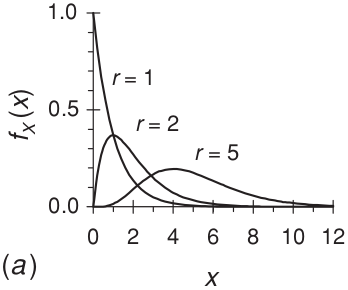
\includegraphics[width=0.8\linewidth]{fi424a.png}  % from Kotte      
\end{minipage}
\hfill
\begin{minipage}{0.49\textwidth}
\centering
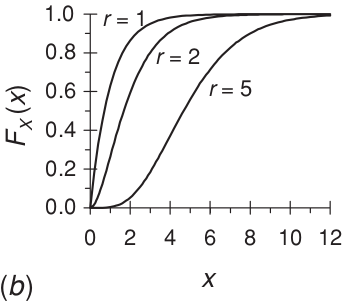
\includegraphics[width=0.8\linewidth]{fi424b.png} % from Kotte
\end{minipage}
\end{frame}

\begin{frame}{Continuous probability distributions} 
    \begin{block}{The \alert{Gamma} distribution}
        The $\Gamma (k)$ function is widely used as the \emph{incomplete gamma function} as:
\[
\Gamma (k,x) =
\begin{cases}
    \int_0^x u^{k-1} e^{-u} du & \text{for } k > 0 \\
    0 & \text{otherwise }
\end{cases}
\]
This can be used to evaluate the gamma \emph{cdf}:
\[
F_X (x) =
\begin{cases}
    \int_0^x f_X (X) dx = \frac{\Gamma (k, \lambda x)}{\Gamma (k)} & \text{for } x \geq 0 \\
    0 & \text{otherwise }
\end{cases}
\]
It has been found that empirical distributions of many natural and non-natural processes that take positive values closely resemble \emph{gamma distribution}. This distribution has been implemented to describe phenomena such as maximum stream flows and the depth of monthly precipitation. In statistics, the \emph{gamma distribution} is important because the \alert{chi-squared distribution} is a particular form of the gamma with $k=\nu /2$, where $\nu$ are the degrees of fredom, and $\lambda = 1/2$. The \emph{cdf} of the \emph{chi-squared distribution} is:
\[
    F (\chi^2) = \frac{1}{2} \int_0^{\chi^2} \frac{(t/2)^{(\nu/2)-1} e^{-t/2}}{\Gamma (\nu/2)} dt
\]
where $t$ is a dummy variable.
    \end{block}
\end{frame}

\begin{frame}{Continuous probability distributions} 
 \begin{exampleblock}{Maximum flows}
     Based on a histogram of data of maximum annual river flows in the Weldon River, USA, between 1930 and 1960, it was assume that the data followed a \emph{gamma pdf}. The parameters were estimated and equal to $k= 1.727$ and $\lambda = 0.00672$ cfs$^{-1}$. According to these values, $\mu_X = \frac{k}{\lambda} = \frac{1.727}{0.00672} = 256.7$ cfs, $\sigma_X  = \frac{\sqrt{k}}{\lambda} = 190$ cfs. Also, the probability that the maximum flow is less than 400 cfs in any year is $F_X (400) = \frac{\Gamma (1.727, \lambda 400}{\Gamma (1.727)} = \frac{0.71}{0.914} = 0.78$. No that the values to estimate the numerator and denominator are taken from tables of the gamma function. 
    \end{exampleblock}
\end{frame}

\begin{frame}{Continuous probability distributions} 
    \begin{block}{The \alert{Beta} distribution}
        The \alert{Beta distribution} is uses to model a random variable whose values go from  0 to 1, and thus it is important in decision methods. The \emph{beta pdf}  is given by: 
\[
f_X (x) =
\begin{cases}
    \frac{1}{B(\alpha, \beta)} x^{\alpha-1} (1-x)^{\beta -1}  & \text{for } 0 < x < 1 \\
    0 & \text{otherwise }
\end{cases}
\]
where $\alpha$ and $\beta$ are parameters that $\alpha > 0$ and $\beta > 0$, and:
\[
    B(\alpha, \beta) = \int_0^1 x^{\alpha -1} (1-x)^{\beta-1} dx = \frac{\Gamma (\alpha) \Gamma (\beta)}{\Gamma (\alpha + \beta)}
\]
From this two equations, the nth moment is:
\[
E[X^n] = \frac{B(\alpha + n, \beta)}{B(\alpha, \beta)}
\]
Considering that $\Gamma (k+1)= k\Gamma (k))$ and using this equation, we have:
\[
    E[X] = \frac{\alpha}{\alpha + \beta}
\]
Similarly, considering that $\Gamma (k+2) = (k+1)\Gamma (k+1)=(k+1)k\Gamma(k) $ and simplifying,
\[
    Var[X] = E[X^2] - \left( E[X] \right)^2 = \frac{\alpha \beta}{(\alpha + \beta)^2 (\alpha + \beta +1)}
\]

               \end{block}
\end{frame}

\begin{frame}{Continuous probability distributions} 
    \begin{block}{The \alert{Beta} distribution}
        The following figures show the \emph{pdf} and the \emph{cdf} for different combinations of $\alpha$ and $\beta$.
               \end{block}
   \vspace{-5pt}
\begin{minipage}{0.49\textwidth}
\centering
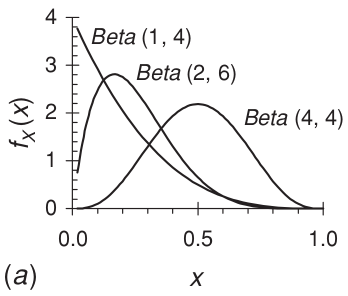
\includegraphics[width=0.8\linewidth]{fi425a.png}  % from Kotte      
\end{minipage}
\hfill
\begin{minipage}{0.49\textwidth}
\centering
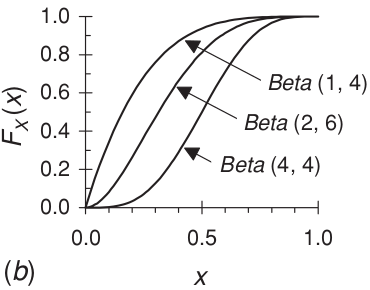
\includegraphics[width=0.8\linewidth]{fi425b.png} % from Kotte
\end{minipage}
Note that when $\alpha = \beta$ the \emph{pdf} is symmetrical and when $\alpha=\beta=1$ is equivalent to the \emph{uniform distribution} with $a=0$ and $b=1$.
\end{frame}

\begin{frame}{Continuous probability distributions} 
    \begin{block}{The \alert{Weibull} distribution}
        The \alert{Weibull distribution} approximate closely to many natural phenomena. It has been used to model, for instance, the time to failure of electrical and mechanical systems. The \emph{pdf} is defined as:
\vspace{-5pt}
 \[
f_X (x) =
\begin{cases}
    \frac{\beta}{\lambda} \left( \frac{x}{\lambda} \right)^{\beta -1} e^{-\left( \frac{x}{\lambda} \right)^{\beta}}, & \text{for } x > 0  \\
    0 & \text{otherwise }
\end{cases}
\]
And the \emph{cdf} takes the form:
\vspace{-5pt}
 \[
F_X (x) =
\begin{cases}
    f_X (x) = \frac{\beta}{\lambda} \left( \frac{x}{\lambda} \right)^{\beta -1} e^{-\left( \frac{x}{\lambda} \right)^{\beta}}, & \text{for } x > 0  \\
    0 & \text{otherwise }
\end{cases}
\]
where $\lambda > 0$. The figures below show the \emph{pdf} and \emph{cdf} for different values of $\beta$ and $\lambda = 1$.
\end{block}
\vspace{-5pt}
\begin{minipage}{0.49\textwidth}
\centering
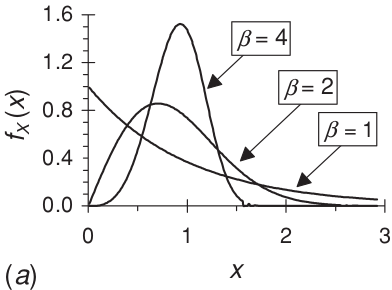
\includegraphics[width=0.8\linewidth]{fi426a.png}  % from Kotte      
\end{minipage}
\hfill
\begin{minipage}{0.49\textwidth}
\centering
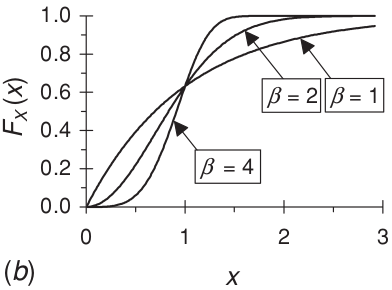
\includegraphics[width=0.8\linewidth]{fi426b.png} % from Kotte
\end{minipage}
Note than from the definition of the \emph{pdf} and \emph{cdf}, if a random variable $X \sim \text{ Weibull } (\beta, \lambda)$, then $Y = \left( X/\lambda \right)^{\beta} \sim \text{ exponential } (\lambda=1)$, $f_Y (y) = e^{-y}$. 
\end{frame}

\begin{frame}{Continuous probability distributions} 
    \begin{block}{The \alert{Weibull} distribution}
        \begin{itemize}
            \item \emph{mean}
                \[
                    E[X] = \lambda \Gamma \left( 1 + \frac{1}{\beta} \right)
                \]
            \item \emph{variance}
                \[
                    Var[X] = E[X^2] - \left( E[X] \right)^2 = \lambda^2 \left[ \Gamma \left(1 + \frac{2}{\beta} \right) - \left( \Gamma \left( 1 + \frac{1}{\beta} \right) \right)^2 \right]
                \]
        \end{itemize}
        Note that for $\beta=1$ the \emph{Weibull pdf} becomes the \emph{exponential pdf}.
\end{block}
 \begin{exampleblock}{Estimation of low flows} % from Kotte
     From a ten-years daily average streamflow time series  in \emph{cfs} at the River Pang at Pangbourne 10-days averages are estimated. From this new aggregated time series, the minimum annual 10-days average flows are estimated. The ranked values are: $13.4 \quad 25.7 \quad 32.2 \quad 35.9 \quad 40.0 \quad 40.0 \quad 40.4 \quad 50.7 \quad 58.2 \quad 71.4$. Regarding that  the \emph{Weibull distribution} is associated with the \emph{extreme value theory}, the distribution can be applied to minima. Estimating the \emph{mean} and the \emph{variance} from the data and using the equations yield by the method of moments (see the equations above), one can resolve this two equations iteratively for the shape parameter $\beta$ and for the scale parameter $\lambda$. Alternatively, the \emph{methods of likelihood} can be used iteratively. An alternative procedure is to used the \emph{least-squares procedure} from the \emph{cdf}. So from the \emph{cdf}:
     \[
         \ln (x_i) - \ln (\lambda) = \frac{\left[\ln \left[-\ln \left(1 - F_X (x_i) \right) \right]\right]}{\beta}
     \]
    \end{exampleblock}
\end{frame}

\begin{frame}{Continuous probability distributions} 
 \begin{exampleblock}{Estimation of low flows} % from Kotte
     Applying the plotting position, which is the probability at which $x_i$ should be plotted, we have $F_X (x_i) = \frac{(i-0.35)}{n}$, and letting $z_i = \ln (x_i)$ and $ y_i= \ln \left[-\ln \left(1 - F_X (x_i) \right) \right]$, we obtain:
\vspace{-5pt}
     \[
         z_i = \frac{y_i}{\beta} + \ln (\lambda) + \epsilon
     \]
     where $i$ is the rank of the data in ascending order, $n$ is the number of data values and $\epsilon$ is an error term in the regression. Applying the least-square fit to this equation for $n=10$:
\vspace{-5pt}
     \[
         \hat{\beta} = \frac{\sum_{i=1}^{n=10} \left( y_i - \bar{y} \right)^2}{\sum_{i=1}^{n=10} \left( y_i - \bar{y} \right) \left(z_i - \bar{z} \right)} = 2.59
     \]
     and
\vspace{-5pt}
     \[
     \hat{\lambda} = e^{\left( \bar{z} - \bar{y}/\hat{\beta}\right)} = 44.85 \, m^3/s
 \]
 where $\bar{z} = \frac{1}{10}\sum_{i=1}^{n=10} z_i $ and $\bar{y} = \frac{1}{10}\sum_{i=1}^{n=10} y_i $. This linear relationship between $z$ and $y$ represent the least-squares fit  of the data  to the two-parameter  \emph{Weibull distribution} (see figure).

\vspace{-5pt}
\begin{minipage}{0.39\textwidth}
\centering
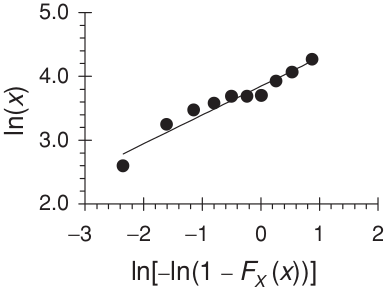
\includegraphics[width=1\linewidth]{fi427.png}  % from Kotte      
\end{minipage}
\hfill
\begin{minipage}{0.59\textwidth}
     The approximate lower 99\% confidence limit for $\beta$ is $\frac{\hat{\beta}}{2n} x_{2n,0.99}^2 = \frac{2.59}{20} 8.26 = 1.07$. Also, quantile estimates can be obtained using the estimates of the Weibull parameters and the preceding equations. For example the annual minimum 10-day flow with a return period of 10 yrs is: 
\vspace{-5pt}
     \[
         y_{10} = \ln \left[ - \ln \left( 1-\frac{1}{10} \right) \right] = -2.25
         \]
\vspace{-7pt}
         \[
             x_{10} = e^{\left[ \left( \frac{y_{10}}{\hat{\beta}} \right) +\ln (\hat{\lambda}) \right]} = 18.8\, m^3/s
         \]

\end{minipage}
   \end{exampleblock}
\end{frame}

\begin{frame}{Continuous probability distributions} 
    \begin{block}{The \alert{Normal} distribution}
The \alert{Normal or Gauss distribution} originally emerged in the study of \emph{experimental errors}. This errors are differences between observations recorded under unchanged similar experimental conditions. In telecommunications, errors are used to be known as \emph{noise}, which  is, in general, the difference between the true estate and the observation. The \alert{Normal distribution} is thus ideal to represent such error when they are of an additive nature. The \emph{pdf} of the \alert{Normal distribution} of a random variable $X$ is:
        \[
            f_X (x) = \frac{1}{\sigma \sqrt{2\pi}} e^{\left[-\frac{1}{2}\left( \frac{x-\mu}{\sigma} \right)^2 \right]}, \text{ for } -\infty < x < \infty
        \]
    This \emph{pdf} is especified by two parameters: the mean or location parameter ($\mu$) and the standard deviation or scale parameter ($\sigma$), computed from the population. In practices, it is common to use the standardized  curve with the transformation of $X$ into $Z$ as $Z=\frac{X-\mu}{\sigma}$, so the \emph{pdf} is:
\vspace{-6pt}
        \[
            f_Z (z) = \frac{1}{\sigma \sqrt{2\pi}} e^{\left(-\frac{1}{2}z^2 \right)}
        \]

\vspace{-20pt}
\begin{minipage}{0.59\textwidth}
        When $\mu=0$ and $\sigma=1$, the \emph{pdf} is:
\vspace{-6pt}
        \[
            f_Z (z) = \frac{1}{\sqrt{2\pi}} e^{\left(-\frac{1}{2}z^2 \right)}
        \]
\end{minipage}
\hfill
\begin{minipage}{0.39\textwidth}
\centering
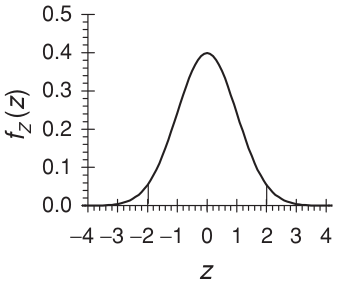
\includegraphics[width=0.9\linewidth]{fi429.png}  % from Kotte      
\end{minipage}

    \end{block}
                
\end{frame}

\begin{frame}{Continuous probability distributions} 
    \begin{block}{The \alert{Normal} distribution}
        \vspace{-4pt}
        Note that the \emph{cdf} can only be calculated using numerical methods and it is:
        \vspace{-5pt}
            \begin{align*}
                F_X (x) &= Pr[X \leq x] = Pr\left[ Z \leq \frac{X-\mu}{\sigma} \right] = Pr [Z \leq z] \\
                        &=\int_{-\infty}^z \frac{1}{\sqrt{2\pi}} e^{- \left(\frac{u^2}{2}\right)} du, \, \text{for } -\infty < z < \infty  
            \end{align*}
            Because of the symmetry of the \emph{pdf}, $f_Z(-z) = 1-f_Z(z)$. Below, some properties of the normal distribution:
        \vspace{-3pt}
        \begin{itemize}
            \item A linear transformation $Y = bX +a$  of a random variable $X$ with $N\sim(\mu,\sigma^2)$ makes $Y$ an  $N\sim(b\mu +a,b^2 \sigma^2)$ random variable. 
            \item If $X_i$ $i=1,2, \cdots, n$ are independent and identically distributed random variables from a population with mean $\mu$ and standard deviation $\sigma$, then the random variable $\bar{X}_n = \sum_{i=1}^n \frac{X_i}{n}$ that is the sample mean, from a random sample of size n from the sample population, tends to have  an $N\sim(\mu,\sigma^2 /n)$ distribution as $n \rightarrow \infty$. This important results is called the \alert{central limit theorem}. The theorem states that even if the distribution of the random variable $X_i$ is nor normal, the so called sampling distribution of its mean will tend to normality asymptotically. 
            \item If $X$ and $Y$ are independent random variables normally distributed with $\mu_X$ and $\mu_Y$, and $\sigma_X^2$ and  $\sigma_Y^2$, respectively, the expression $Z=X+Y$ is normally distributed too with $\mu_Z = \mu_X + \mu_Y$ and $\sigma_Z^2 = \sigma_X^2 + \sigma_Y^2$. This is also applicable for $Z = X-Y$ with $\mu_Z = \mu_X - \mu_Y$ and $\sigma_Z^2 = \sigma_X^2 + \sigma_Y^2$. If $X$ and $Y$ are not statistically independent but correlated, $Z$ is still normally distributed bu $\sigma_Z^2 = \sigma_X^2 + \sigma_Y^2 + 2\rho \sigma_X \sigma_Y$, where $\rho$ is the linear correlation between $X$ and $Y$.
        \end{itemize}
    \end{block}
                
\end{frame}

\begin{frame}{Continuous probability distributions} 
 \begin{exampleblock}{Streamflows} % from Diaz-Gra
     Annual average discharges in river $X$ are distributed following a $N \sim (400,50^2)$.Annual average discharges of a tributary $Y$ of river $X$ are distributed as $N \sim (145, 76^2)$.  Downstream of the mouth of river $Y$, there is an outflow $D$ to supply water to agricultural fields. Downstream of $D$, annula avearge discharges in river X are distributed as $N \sim (425, 91.5^2)$. Assuming that $X$, $Y$ and $D$ are independent, the \emph{pdf} of annual average discharges in $D$ is normal with $\mu_D = 300 + 145 - 425 = 20$ and $\sigma_D^2 =91.5^2 - 76^2 - 50^2 = 9.81^2 $. The probability that $D>30$ can be estimated as $z=\frac{30-20}{9.81} = 1.0194$ and $F_Z (z=1.0194)=0.846$. So the $Pr[D > 30] = 1-0.846 = 0.154$. If $X$, $Y$ and $D$ are not independent and $\rho_{X,Y} = 0.15$ and $\rho_{X,D} = -0.35$ (under the assumption that that the lower the streamflow in $X$ the greater the flow derived by $D$), $\mu_D = 20$ and $91.5^2 = 97.0261^2 + \sigma_D^2 - 2 (-0.35)(97.0361)\sigma_D$, from where $\sigma_D^2 = 23.49^2$. For this case, the $Pr[D>30] = 0.3352$. 

 \end{exampleblock}
               
\end{frame}


\begin{frame}{Continuous probability distributions} 
    \begin{block}{The \alert{Lognormal} distribution}
        We know that the addition of large number of small random effects will tend to make the distribution of the aggregate approach normal. In contrast, if the phenomena arises from the multiplicative effect of a large number of uncorrelated factors, the distribution tend to be \alert{Lognormal}, that is, the logarithm of a random variable $X$ becomes normally distributed. Phenomena such as the particle size of sediment samples are \emph{Lognormal}, and the interarrival times of earthquakes. As this distribution of defined for non-negative values is used to describe daily average streamflows, maximum streamflows, and daily, monthly and annual rainfall. If $X$ is a positive random variable, then $Y = \ln (X)$. Accordingly, if $Y$ has $N \sim (\mu_Y , \sigma_{Y^2})$, $X$ has a \emph{Lognormal distribution} $LN \sim (\mu_{\ln(X)}, \sigma_{\ln(X)}^2)$. So the \emph{pdf} is:
        \[
            f_X (x) = \frac{1}{x \sigma_{\ln (X)} \sqrt{2\pi}} e^{\left[ -\frac{1}{2} \left[ \frac{\ln (X) -\mu_{\ln (X)}}{\sigma_{\ln (X)}} \right]^2 \right]}, \, \text{for } 0 \leq x < \infty
            \]
            See the figure below with plot of the \emph{Lognormal pdf}.
   \end{block}

\begin{minipage}{0.37\textwidth}
\centering
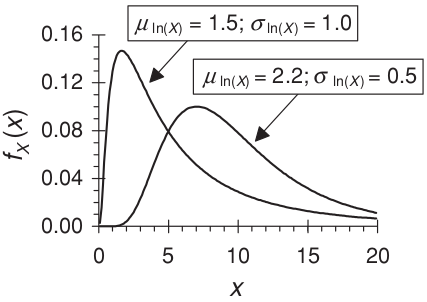
\includegraphics[width=0.95\linewidth]{fi4210.png}  % from Kotte      
\end{minipage}
\hfill
\begin{minipage}{0.59\textwidth}
    The expectation operator can be written as: 
    \begin{align*}
        E\left[X^r \right] &= \int_0^{\infty} x^r f_X (x) dx  \\
        &= \frac{1}{\sigma_{\ln (X)} \sqrt{2\pi}} \int_{-\infty}^{\infty} e^{ry} e^{\left[ -\frac{1}{2} \left[ \frac{ y-\mu_{\ln (X)}}{\sigma_{\ln (X)}} \right]^2 \right]} dy
    \end{align*}
\end{minipage}
                
\end{frame}

\begin{frame}{Continuous probability distributions} 
    \begin{block}{The \alert{Lognormal} distribution}
        From where $E \left[X^r \right] = E\left[ e^{Yr} \right]; Y \sim N\left( \mu_{\ln(X)]}, \sigma_{\ln(X)}^2 \right)$, so $E \left[X^r \right] = M_Y (r) = e^{r\mu_{\ln(X)} + \frac{1}{2} r^2 \sigma_{\ln(X)}^2}$. Thus , the \emph{mean} is:
        \[
        \mu_X = E[X] = e^{\left[ \mu_{\ln(X)} + \frac{1}{2} \sigma_{\ln(X)}^2 \right]} 
    \]
     and the \emph{variance} is:
    \vspace{-9pt}
        \[
            \sigma_X^2 = E[X^2] - \mu_X^2 = e^{2\left[ \mu_{\ln(X)} + \sigma_{\ln(X)}^2 \right]} - e^{2\left[ \mu_{\ln(X)} + \frac{1}{2} \sigma_{\ln(X)}^2 \right]} = \mu_X^2 \left( e^{\left[ \sigma_{\ln(X)}^2\right]}  - 1 \right)
    \]
    When the \emph{Lognormal distribution} is defined upon an $a$ value, this is called the three-parameters Lognormal distribution or the \alert{Gibrat-Galton distribution}, that is, $LN (a, \mu_{\ln(X)}, \sigma_{\ln(X)}^2$. Accordingly, the transformation becomes $Y = \ln(X-a)$ so the \emph{pdf} is:
    \vspace{-9pt}
    \[
            f_X (x) = \frac{1}{(x-a) \sigma_{\ln (X-a)} \sqrt{2\pi}} e^{\left[ -\frac{1}{2} \left[ \frac{\ln (X-a) -\mu_{\ln (X-a)}}{\sigma_{\ln (X-a)}} \right]^2 \right]}, \, \text{for } a \leq x < \infty
        \]
        where the \emph{mean} is:
    \vspace{-9pt}
        \[
            \mu_{\ln(X-a)} = \ln \left(\mu_X -a \right) - \frac{1}{2} \ln \left[ 1 + \left( \frac{\sigma_X}{\mu_X -a} \right)^2 \right]
        \]
        and the \emph{variance} is:
    \vspace{-9pt}
        \[
        \sigma_{\ln(X-a)}^2 = \ln \left[ 1 + \left( \frac{\sigma_X}{\mu_X -a} \right)^2 \right]
    \]
   \end{block}
\end{frame}

\begin{frame}{Some discrete and continuous probability density functions} 
    \centering
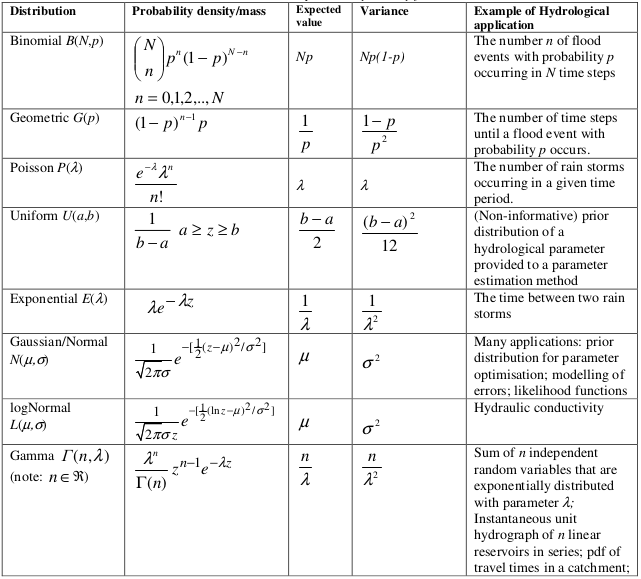
\includegraphics[width=0.91\linewidth]{taBi32a.png}  % from Bierk
\end{frame}

\begin{frame}{Some discrete and continuous probability density functions} 
    \centering
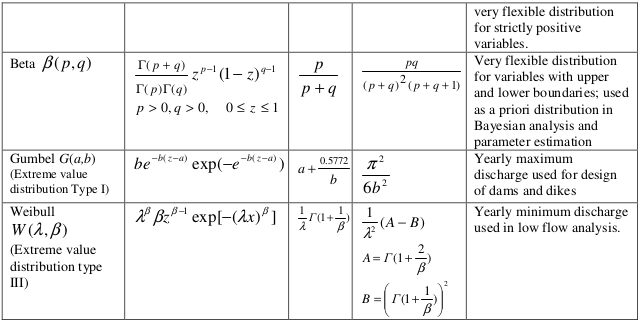
\includegraphics[width=0.95\linewidth]{taBi32b.png}  % from Bierk
\end{frame}

\begin{frame}{Characteristics functions of some  probability distributions} 
    \centering
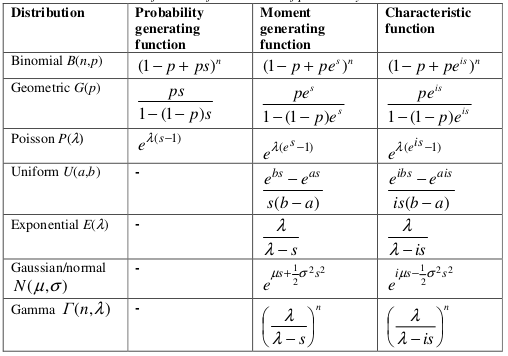
\includegraphics[width=0.95\linewidth]{taBi33.png}  % from Bierk
\end{frame}




\subsection{Multivariate distributions} %% From  Kotte
\begin{frame}{Multivariate distributions} 
    Here, the multivariate type of distribution is examined for jointly distributed random variables. For instance the exponentially distributed storm intensity and duration lead to a \emph{bivariate exponential distribution} or intensity and duration considering the correlation between these two variables. While the \emph{bivariate normal distribution} is examined in detail other types are discussed briefly.
    \begin{block}{The \alert{Bivariate normal} distribution}
        The \emph{joint distribution} of two random variables $X$ and $Y$, each normally distributed is called the \alert{bivariate normal distribution}. The \emph{pdf} in standardized form is given for $Z_1$ and $Z_2$ as:
        \vspace{-15pt}
        \[
            f_{Z_1 , Z_2} (z_1 , z_2) = \left[ 2\pi \left( 1- \rho^2 \right)^{1/2} \right]^{-1} e^{\left[ \frac{-\left( z_1^2 - 2\rho z_1 z_2 + z_2^2 \right)}{\left( 2- 2\rho^2 \right)} \right]}, \, \text{for } -\infty < z_1 , z_2 < \infty
            \]
            where $r$, $-1 \leq \rho \leq 1$, is linear correlation coefficient between the two variables. Note also that $Z_1 = \frac{X - \mu_X}{\sigma_X}$ and $Z_2 = \frac{Y - \mu_Y}{\sigma_Y}$ where $-\infty < \mu_X , \mu_Y < \infty$ and $\sigma_X , \sigma_Y > 0 $. In terms of $X$ and $Y$ ($-\infty < x , y < \infty$) the \alert{bivariate normal distribution} is:
        \vspace{-5pt}
        \[
            f_{X , Y} (x , y) = \frac{1}{2 \pi \sigma_X \sigma_Y \sqrt{1- \rho^2}} e^{\left[ -\frac{1}{2(1-\rho^2)} \left[ \left(\frac{x-\mu_X}{\sigma_X}\right)^2 - 2\rho \frac{x-\mu_X}{\sigma_X} \frac{y-\mu_Y}{\sigma_Y} +  \left(\frac{y-\mu_Y}{\sigma_Y}\right)^2 \right] \right]}             
        \]
   \end{block}
   \vspace{-15pt}
\begin{minipage}{0.37\textwidth}
\centering
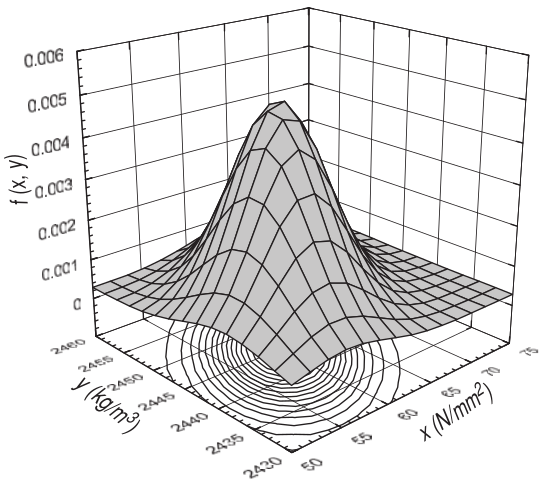
\includegraphics[width=0.8\linewidth]{fi431.png}  % from Kotte      
\end{minipage}
\hfill
\begin{minipage}{0.59\textwidth}
    This figure shows the relationship of compressive strength and density in concrete. In general, the bivariate distribution shows how upon one variable is possible to predict the performance of another. 
\end{minipage}

\end{frame}

\begin{frame}{Multivariate distributions} 
    \begin{block}{The \alert{Bivariate exponential} distribution}
        There are many others useful bivariate distribution, this is case of the \alert{bivariate exponential distribution} whose \emph{cdf} is:
        \[
            F_{X,Y} (x,y) = 1-e^{-ax} - e^{-by} - e^{-ax - by - cxy}, \, \text{for } x,y \geq 0 
        \]
        where $a,b,c > 0$ are parameters of the distribution. 
   \end{block}
 \begin{block}{The \alert{Bivariate logistic} distribution}
     The \emph{cdf} of the \alert{bivariate logistic distribution} in its basic form is:
        \[
            F_{X,Y} (x,y) = \left( 1 + e^{-x} + e^{-y} \right)^{-1}, \, \text{for } x,y \geq 0
        \]
   \end{block}

        \end{frame}


\end{document}

